\chapter{One-dimensional finite-volume methods}
\label{chp-1d-fv}

\theoremstyle{plain}
\newtheorem{lema}{Lemma}[chapter]

\theoremstyle{plain}
\newtheorem{prop}{Proposition}[chapter]

\theoremstyle{plain}
\newtheorem{remark}{Remark}[chapter]

\theoremstyle{plain}
\newtheorem{corollary}{Corollary}[chapter]

\theoremstyle{plain}
\newtheorem{definition}{Definition}[chapter]


The aim of this chapter is to give a detailed description of the celebrated
Piecewise-Parabolic Method (PPM) proposed by \citet{colella:1984}.
As we shall see, the PPM is a one-dimensional finite-volume method for
hyperbolic conservation laws that at each time step requires two tasks. 
The first task may be stated as: given the estimates of average values of the
conservation laws solution, find a Piecewise-Parabolic function that approximates 
the function and preserves its local integral value (also referred as local mass).
The second task is the following: given the Piecewise-Parabolic approximation 
(also known as reconstruction), solve the conservation law using the parabolas 
to obtain the solution at the next time-step.
For instance, if the conservation law is the advection equation, the second step
consists of advecting the parabolas.
In the first step, we may also require some monotonization constraints on the parabolas,
to ensure that no new extreme value is created in the Piecewise-Parabolic reconstruction, 
ensuring that the scheme is free of numerical oscillations.
The steps required for PPM make it an REA (reconstruct, evolve, and average) algorithm,
or also referred to as a Godonuv-type method, which was originally proposed by 
\citet{godunov:1959}.

The PPM approach has become popular in the literature for gas 
dynamics simulations, astrophysical phenomena modeling \citep{woodward:1986}
and later on atmospheric simulations \citep{carpenter:1990}.
Indeed, the PPM has been implemented in the FV3 dynamical core on its 
latitude-longitude grid \citep{lin:2004} and cubed-sphere \citep{putman:2007}
versions.
We point out that the reconstruction function may be built using other basis 
functions rather than parabolas. In fact, PPM may be thought of as an extension of 
the Piecewise-Linear method from \citet{vanleer:1977}, which, on the other hand,
was inspired by the Piecewise-Constant method attributed to \citet{godunov:1959}.
Besides that, other schemes inspired by PPM were proposed in the literature using
higher-order polynomials, such as quartic polynomials \citep{white:2008}.
For a review of general piecewise-polynomial reconstruction we refer 
to the technical report from \citet{engwirda:2016}, \citet{lauritzen:2011}
and the references therein.
Even though many other shapes for the basis functions are available in the 
literature, as well higher order schemes, \citet{harris:2021} points out that the PPM
scheme suits well the FV3 needs in the sense of being a flexible method 
that can be modified to ensure low diffusivity or shape-preservation, for example.
Besides that, a finite-volume numerical method usually requires
monotonicity constraints, which by Godunov's theorem, limits 
the order of convergence to at most 1.
So, a higher-order scheme needs to be well-balanced on the trade-off between 
computational cost increasing and potential benefits.


This chapter starts with a basic review of one-dimensional conservation laws in
the integral form in Section \ref{chp2-sec1}, and in Section \ref{chp2-sec2} 
we set the framework of general one-dimensional finite-volumes schemes,
where we also introduce concepts such as consistency, convergence and stability.
Section \ref{chp2-sec-ppm} describes the PPM method and its convergence order analysis
of its reconstruction in given in Subsection \ref{chp2-sec-recon}.
Subsection \ref{chp2-sec-mono} is dedicated to introducing possible ways to monotonizate
the parabolas.
Subsection \ref{chp2-sec-flux} is dedicated to the description and investigation of the PPM flux
computation considering the one-dimensional advection equation as the conservation law.
Section \ref{chp2-sec-numerical-exp} shows some numerical results using the PPM scheme
for the advection equation.  At last, Section \ref{chp2-sec-conclusion} presents
some conclusions.
The usage of PPM to solve two-dimensional problems
will be addressed in Chapter \ref{chp-2d-fv}.

\section{One-dimensional system of conservation laws in integral form}
\label{chp2-sec1}
In this section, we are going to present the derivation of one-dimensional 
system of conservation laws in the integral form. 
The derivation presented here follows \citet{leveque:1990} and \citet{leveque:2002} closely and will
be useful to fix some notation. \index{Conservation law}
Let us assume that $x$ and $t$ represent the spatial and time coordinates, respectively.
Given $[x_1, x_2] \subset \mathbb{R}$, $x_1 \leq x_2$, and a time 
interval $[t_1, t_2] \subset ]0, +\infty[$, $t_1 \leq t_2$, 
we aim to describe how $m$ state variable densities given by functions 
$q_1, \cdots, q_m: \mathbb{R}\times[0, +\infty[ \to \mathbb{R}$ 
evolve within time in the considered time interval, assuming that we have neither sinks nor sources 
for the mass of each state variable and also assuming that the mass
flow rate is known for all the state variables.

To set the problem in more mathematical terms, let us denote by 
${q}: \mathbb{R}\times [0, +\infty[\to \mathbb{R}^m$, 
${q} = {q}(x,t)$, the vector of state variables,
\textit{i.e.}, ${q}_k = q_k$ for $k=1, \cdots, m$.
The mass of ${q}$ in $[x_1, x_2]$ at time $t$ is defined by:
\begin{equation}
	\label{chp2-sec1-eq1}
	{M}_{[x_1, x_2]}(t) := \int_{x_1}^{x_2} {q}(x,t) \,dx \in \mathbb{R}^m.
\end{equation}

Thus, the mass in $[x_1, x_2]$ of the $k$-th state variable $q_k$ is equal to
$({M}_{[x_1, x_2]}(t))_k$, $\forall k = 1, \cdots, m$.
We are going to assume the following physical constraints concerning the total mass of each state variable:
\begin{enumerate}
	\item No mass is created;
	\item No mass is destroyed.
\end{enumerate}

Also, let us assume that the mass flow rate in a point $x$ and at a time 
$t > 0$ is given by ${f}({q}(x,t))$, where ${f}:\mathbb{R}^m \to \mathbb{R}^m$ is 
a continuously differentiable ($\mathcal{C}^1$) function. This function ${f}$ is known as flux function.
With the physical constraints that we imposed, the following equation must hold for the mass:
\begin{equation}
	\label{chp2-sec1-eq2}
	\frac{d}{dt} \bigg( \int_{x_1}^{x_2} {q}(x,t) \,dx \bigg) = 
	{f}({q}(x_1,t)) - {f}({q}(x_2,t)) .
\end{equation}
Equation \eqref{chp2-sec1-eq2} is known as a conservation law written in integral form and tell us how the mass 
${M}_{[x_1, x_2]}(t)$ varies with time. Another integral form of the conservation law may be obtained integrating
Equation \eqref{chp2-sec1-eq2} with respect to time in $[t_1, t_2]$ leading to: \index{Conservation law !in integral form}
\begin{equation}
	\label{chp2-sec1-eq3}
	\int_{x_1}^{x_2} {q}(x, t_2) \,dx = 
	\int_{x_1}^{x_2} {q}(x, t_1) \,dx + 
	\int_{t_1}^{t_2} {f}({q}(x_1, t)) \,dt -
	\int_{t_1}^{t_2}{f}({q}(x_2, t)) \,dt .
\end{equation}

Assuming that ${q}$ is a $\mathcal{C}^1$ function, we may write:
\begin{equation}
	\label{chp2-sec1-eq4}
	\int_{t_1}^{t_2} 
	\frac{\partial}{\partial t} {q}(x,t) \,dt
	= {q}(x, t_2) - {q}(x, t_1) ,
\end{equation}
and
\begin{equation}
	\label{chp2-sec1-eq5}
	\int_{x_1}^{x_2} \frac{\partial}{\partial x}{f}({q}(x,t)) \,dx 
	= {f}({q}(x_2, t)) -
	{f}( {q}(x_1, t)) .
\end{equation}

Replacing Equations \eqref{chp2-sec1-eq4} and \eqref{chp2-sec1-eq5}
in \eqref{chp2-sec1-eq3} we get the differential form of the conservation law:
\index{Conservation law !in differential form}
\begin{equation}
	\label{chp2-sec1-eq6}
	\int_{t_1}^{t_2} \int_{x_1}^{x_2} 
	\bigg( \frac{\partial}{\partial t}{q}(x, t) 
	+ \frac{\partial}{\partial x} {f}({q}(x, t)) \bigg) 
	\,dx \,dt  = 0.
\end{equation}

Since Equation \eqref{chp2-sec1-eq6} must hold for all $x_1, x_2, t_1$ and $t_2$ such that
$[x_1, x_2] \times [t_1, t_2] \subset \mathbb{R}\times ]0, +\infty[$, we obtain the differential form of the conservation law:
\begin{equation}
	\label{chp2-sec1-eq7}
	\frac{\partial}{\partial t}{q}(x, t) +
	\frac{\partial}{\partial x} {f}({q}(x, t))
	= 0, \quad \forall (x,t) \in \mathbb{R}\times ]0, +\infty[. 
\end{equation}

We shall assume that the eigenvalues of the Jacobian matrix of the flux function
$D{f}(q)$ are all real and that $D{f}(q)$ is a diagonalizable matrix,
$\forall q \in \mathbb{R}^m$, so that Equation \eqref{chp2-sec1-eq7}
is a hyperbolic partial differential equation \citep{leveque:1990}. As we will 
specify latter, some initial conditions will also be supposed to be known as well.

Many physically relevant equations may be written as Equation \eqref{chp2-sec1-eq7}.
Some examples are the Euler equations for gas dynamics, obtained when $m = 3$,
and the one-dimensional shallow-water equations, obtained $m = 2$.
Other relevant equation is the Burgers equation, which is obtained when
$m = 1$ and $f(q) = q^2$. The Burgers equation is well known for developing shocks,
even for smooth initial conditions, and is a simple prototype to study shock formation.
At last, the linear advection equation is another interesting example, which is obtained
when $m = 1$ and $f(q(x,t)) = u(x,t)q(x,t)$, where $u(x,t)$ is a given velocity.
Strictly speaking, the linear advection is not in the form given by the Equation
\eqref{chp2-sec1-eq7} since $f$ depends on $q$ but also on $(x,t)$.
But, one may check that Equation \eqref{chp2-sec1-eq7} is still hyperbolic
in this case. The linear advection equation will play a key role in this work due to its importance
to the development of atmospheric dynamical cores.

We say that ${q}$ is a strong or classical solution to the conservation law \eqref{chp2-sec1-eq7}
if it is $\mathcal{C}^1$ and satisfies the Equation \eqref{chp2-sec1-eq7}.
Applying the steps from Equation \eqref{chp2-sec1-eq3} to Equation \eqref{chp2-sec1-eq7}
in reverse order, one may check that if ${q}$ is a strong solution,
then it satisfies the integral form \eqref{chp2-sec1-eq3} for all $x_1, x_2, t_1$ and $t_2$ such that
$[x_1, x_2] \times [t_1, t_2] \subset \mathbb{R}\times ]0, +\infty[$. 
Therefore, Equations \eqref{chp2-sec1-eq3} and \eqref{chp2-sec1-eq7} are
equivalent when ${q}$ is $\mathcal{C}^1$.
However, the problem \eqref{chp2-sec1-eq3} can be formulated
to functions that are not $\mathcal{C}^1$ and have discontinuities.
More generally speaking, we say that ${q} \in L^{\infty}(D, \mathbb{R}^m)$ 
\footnote{$L^{\infty}(D, \mathbb{R}^m) = \{q: D \to \mathbb{R}^m$
	such that $q$ is bounded.$\}$}
if it satisfies the Equation 
\eqref{chp2-sec1-eq3} for all $x_1, x_2, t_1$ and $t_2$ such that
$[x_1, x_2] \times [t_1, t_2] \subset \mathbb{R}\times ]0, +\infty[$.
It can be shown that this notion of weak solution is equivalent to requiring that \citep{leveque:1990}:
\begin{equation}
	\label{chp2-sec1-eq8}
	\int_{-\infty}^{+\infty} \int_{0}^{+\infty} \bigg(
	\frac{\partial}{\partial t} \phi(x, t){q}(x, t) +
	\frac{\partial}{\partial x} \phi(x ,t){f}({q}(x, t)) 
	\bigg)\,dt \,dx = 
	\int_{-\infty}^{+\infty} \phi(x, 0){q}(x, 0) \,dx  , \quad
\end{equation}
$\forall \phi \in C_{0}^{1}(\mathbb{R}\times[0, +\infty[)$
where $C_{0}^{1}(\mathbb{R}\times[0, +\infty[)$ denotes the set
of all continuously differentiable functions with compact support 
in $\mathbb{R}\times[0, +\infty[$. This formulation of weak solution
is more commonly employed in the construction of Discontinuous Galerkin
methods \citep{nair:2011}.

In order to develop finite-volume methods for a system of conservation laws, it is useful to define the vector of
average values of the state variable vector ${q}$ in the interval $[x_1, x_2]$ at a time $t$ by:
\begin{equation}
	\label{chp2-sec1-eq9}
	{Q}(t) = \frac{1}{\Delta x}
	\int_{x_1}^{x_2} {q}(x,t) \,dx
	\in \mathbb{R}^m,
\end{equation}
where $\Delta x = x_2 - x_1$. The Equation \eqref{chp2-sec1-eq2} may be  rewritten in terms of ${Q}$ as:
\begin{equation}
        \label{chp2-sec1-eq10}
	\frac{d}{dt} {Q}(t) = \frac{1}{\Delta x} 
	({f}({q}(x_1,t)) - {f}({q}(x_2,t))) ,
\end{equation}
and so is Equation \eqref{chp2-sec1-eq3}:
\begin{equation}
        \label{chp2-sec1-eq11}
	{Q}(t_2) =  {Q}(t_1) + 
	\frac{1}{\Delta x}\bigg( \int_{t_1}^{t_2} 
	{f}({q}(x_1, t)) \,dt - 
	\int_{t_1}^{t_2}{f}({q}(x_2, t)) \,dt \bigg).
\end{equation}

To move towards finite volume schemes, we will restrict our attention
to a conservation law in a bounded domain of the form 
$D = [a,b]\times[0,T]$, $a<b$, $T>0$. However, we must 
impose some boundary conditions. One possible way that we will adopt 
in the text are the periodic boundary conditions:
\begin{equation}
	\label{chp2-sec1-eq12}
	{q}(a, t) = {q}(b, t),\quad \forall t \in [0, T].
\end{equation}

Also, we assume that an initial condition $q_0(x) = q(x,0)$, $q_0 \in L^{\infty}([a,b],\mathbb{R}^m)$, is given.
Thus, we have specified a Cauchy problem.
We notice that Equations \eqref{chp2-sec1-eq10} and \eqref{chp2-sec1-eq11}
hold for all $x_1, x_2, t_1$ and $t_2$ such that
$[x_1, x_2] \times [t_1, t_2] \subset D$.
So, let us discretize the domain $D$ and write 
Equations \eqref{chp2-sec1-eq10} and \eqref{chp2-sec1-eq11} in terms of this discretization.
Given a positive integer $N_T$, we define the time step 
$\Delta t = \frac{T}{N_T}$, $t^{n} = n \Delta t$, for $n = 0, 1 ,\cdots, N_T$.
For the spatial discretization, we consider a uniformly spaced partition of $[a, b]$ given by: 
\begin{equation}
	\label{chp2-sec1-eq13}
	[a,b] = \bigcup_{i=1}^N X_i, 
	\text{ where } X_i= [x_{i-\frac{1}{2}}, x_{i+\frac{1}{2}}] \text{ and } 
	a = x_{\frac{1}{2}} < x_{\frac{3}{2}} < \cdots < x_{N-\frac{1}{2}} < x_{N+\frac{1}{2}} = b.
\end{equation}

Each interval $X_i$ is referred to as the control volume. \index{Control volume}
We shall use the notations $\Delta x = x_{i+\frac{1}{2}} - x_{i-\frac{1}{2}}$ 
and $x_i = \frac{1}{2}(x_{i+\frac{1}{2}} + x_{i-\frac{1}{2}})$, $\forall i = 1, \cdots, N$, 
to define the control volume length and centroid, respectively.
We also denote by ${Q}_i(t) \in \mathbb{R}^m$ as the vector of 
average values of state variable vector at time $t$
in the control volume $X_i$, $\forall i = 1, \cdots, N$. Replacing $t_1, t_2, x_1$ and 
$x_2$ by $t^{n}, t^{n+1}, x_{i-\frac{1}{2}}$ and $x_{i+\frac{1}{2}}$,
respectively, in Equation \eqref{chp2-sec1-eq10}, we get:
\begin{equation}
	\label{chp2-sec1-eq14}
	\frac{d}{dt} {Q}_i(t) = \frac{1}{\Delta x}
	({f}({q}(x_{i-\frac{1}{2}},t)) -
	{f}({q}(x_{i+\frac{1}{2}},t))) ,
	\quad \forall i = 1, \cdots, N.
\end{equation}

Similarly, Equation \eqref{chp2-sec1-eq11} becomes:
\begin{equation}
        \label{chp2-sec1-eq15}
	\begin{aligned}
		{Q}_i(t^{n+1}) =  {Q}_i(t^{n}) +
		\frac{1}{\Delta x}\bigg( \int_{t^{n}}^{t^{n+1}}
        	{f}({q}(x_{i-\frac{1}{2}}, t)) \,dt -
		\int_{t^{n}}^{t^{n+1}}{f}({q}(x_{i+\frac{1}{2}}, t)) \,dt \bigg),
       		\\
		\quad \forall i = 1, \cdots, N,
		\quad \forall n = 0, \cdots, N_T-1.
	\end{aligned}
\end{equation}

In order to use a more compact notation, it is helpful to use the following centered difference notation:
\begin{equation}
	\label{chp2-sec1-eq16}
	\delta_x {g}(x_i,t) = 
	{g}(x_{i+\frac{1}{2}},t) - 
	{g}(x_{i-\frac{1}{2}},t),
\end{equation}
for an arbitrary vector valued function ${g}$. 
Using this notation, Equations \eqref{chp2-sec1-eq14}
and \eqref{chp2-sec1-eq15} lead to:
\begin{equation}
        \label{chp2-sec1-eq17}
        \frac{d}{dt} {Q}_i(t) = -\frac{1}{\Delta x}
	\delta_x {f}({q}(x_{i},t))
        \quad \forall i = 1, \cdots, N,
\end{equation}
and
\begin{equation}
        \label{chp2-sec1-eq18}
        {Q}_i(t^{n+1}) =  {Q}_i(t^{n}) -
	\frac{\Delta t}{  \Delta x} \delta _x\bigg( \frac{1}{\Delta t}\int_{t^{n}}^{t^{n+1}}
        {f}({q}(x_{i}, t)) \,dt \bigg),
        \quad \forall i = 1, \cdots, N,
        \quad \forall n = 0, \cdots, N_T-1,
\end{equation}
respectively.
It is worth pointing out that we have made no approximation in Equations
\eqref{chp2-sec1-eq17} and \eqref{chp2-sec1-eq18}. Indeed, if ${q}$ satisfies Equation
$\eqref{chp2-sec1-eq2}$, $\forall [x_1, x_2] \subset [a,b]$ and $\forall t \in [0,T]$,
then Equation \eqref{chp2-sec1-eq17} is just Equation
\eqref{chp2-sec1-eq2} evaluated in the control volumes and written
in terms of the average values ${Q}$. 
Similarly, if ${q}$ satisfies Equation
$\eqref{chp2-sec1-eq3}$, $\forall [x_1, x_2] \times [t_1, t_2] \subset D$,
then Equation \eqref{chp2-sec1-eq18} is just Equation
\eqref{chp2-sec1-eq3} evaluated in the control volumes,
at the time instants $t^{n}$, and written
in terms of the average values ${Q}$.

Notice that in Equation \eqref{chp2-sec1-eq18} we divided and multiplied by $\Delta t$, so that 
we can interpret $\frac{1}{\Delta t}\int_{t^{n}}^{t^{n+1}}
{f}({q}(x_{i}, t)) \,dt $ as a mean-time average flux.
This interpretation is very handy for the derivation of finite-volume schemes.

The formulations given by Equations \eqref{chp2-sec1-eq17} and \eqref{chp2-sec1-eq18} are the cornerstone 
of the development of finite volume methods for conservation laws. 
On the right-hand side of Equation \eqref{chp2-sec1-eq17}, the flux function ${f}$ 
may be discretized leading to an ordinary differential equation (ODE)
that might be solved using classical ODE integrators.
These methods are known as semi-discrete methods \citep{leveque:2002}, since only the spatial coordinate is discretized.
In this work, we shall restrict our attention to methods based on Equation \eqref{chp2-sec1-eq18},
even though the PPM approach is applicable for semi-discrete methods (\textit{e.g.} \ \citet{suresh:1997}).

\section{The finite-volume approach}
\label{chp2-sec2}
We summarize the problem of the system of conservation laws in the integral form 
discussed in Section \ref{chp2-sec1} in Problem \ref{chp2-sec2-prob1}.
For simplicity, hereafter we shall constrain our attention to the one-dimensional advection equation, 
that is, we are going to assume $m=1$ and that the flux function has the form 
$f(q(x,t)) = u(x,t)q(x,t)$, where $u(x,t)$ is the velocity which is assumed to be given.

\subsection{Discretization of the problem}
\theoremstyle{plain} 
\newtheorem{prob}{Problem}[chapter]

\begin{prob}
	\label{chp2-sec2-prob1}
	Given $ D = [a,b] \times [0,T]$, a $\mathcal{C}^1$ velocity function ${u}: D \to \mathbb{R}$,
	we would like to find a weak solution ${q} \in L^{\infty}(D, \mathbb{R})$ 
	of the advection equation in the integral form:
	\begin{equation*}
	        \int_{x_1}^{x_2} {q}(x, t_2) \,dx = 
       		\int_{x_1}^{x_2} {q}(x, t_1) \,dx + 
        	\int_{t_1}^{t_2} {f}({q}(x_1, t)) \,dt -
		\int_{t_1}^{t_2}{f}({q}(x_2, t)) \,dt ,
	\end{equation*}
	$\forall [x_1, x_2]\times[t_1, t_2] \subset D$, 
	given the initial condition 
	${q}(x,0) = {q}_0(x)$, $\forall x \in [a,b]$, 
	assuming periodic boundary conditions, 
	\textit{i.e.}, ${q}(a,t) = {q}(b,t)$, $\forall t \in [0,T]$,
	and $f(q(x,t)) = u(x,t)q(x,t)$.
\end{prob}

We point out that, for Problem \ref{chp2-sec2-prob1}, 
the total mass in $[a,b]$ satisfies: 
\begin{equation}
	{M}_{[a,b]}(t) = {M}_{[a,b]}(0), \quad \forall t \in [0,T].
\end{equation}
This is the conservation of total mass propriety and is highly desirable
for any numerical scheme that intends to give a robust approximation of a
system of conservation laws solution.
In Section \ref{chp2-sec1} we introduced a version of Problem \ref{chp2-sec2-prob1}
considering a discretization of the domain $D$. 
This idea is summarized in Problem \ref{chp2-sec2-prob2}.
\begin{prob}
    \label{chp2-sec2-prob2}
		Assume the framework of Problem \ref{chp2-sec2-prob1}.
    We consider positive integers $N$ and $N_T$, a spatial discretization of [a,b] given by
    $X_i = [x_{i-\frac{1}{2}}, x_{i+\frac{1}{2}}]$,$\forall i = 1, \cdots, N,$ 
		$a = x_{\frac{1}{2}} < x_{\frac{3}{2}} < \cdots < x_{N-\frac{1}{2}} < x_{N+\frac{1}{2}} = b$,
		$\Delta x = x_{i+\frac{1}{2}}-x_{i-\frac{1}{2}}$,
		a time discretization
    $t^{n} = n\Delta t$, $\Delta t = \frac{T}{N_T}$, $\forall n = 0, \cdots, N_T$.
		Since we are in the framework of Problem \ref{chp2-sec2-prob1}, it follows that:
		\begin{equation}
			\label{1d-fvexact-scheme}
						{Q}_i(t^{n+1}) =  {Q}_i(t^{n}) -
						\frac{\Delta t}{\Delta x} \delta _x\bigg( \frac{1}{\Delta t}\int_{t^{n}}^{t^{n+1}}
						{f}({q}(x_{i}, t)) \,dt \bigg),
						\quad \forall i = 1, \cdots, N,
						\quad \forall n = 1, \cdots, N_T-1,
		\end{equation}
		where ${Q}_i(t) = \frac{1}{\Delta x}
		\int_{x_{i-\frac{1}{2}}}^{x_{i+\frac{1}{2}}} {q}(x,t) \,dx$.

		Our problem now consists of finding the values ${Q}_i(t^{n})$, 
		$\forall i = 1, \cdots, N$, $\forall n = 0, \cdots, N_T-1$,
		given the initial values ${Q}_i(0)$, $\forall i = 1, \cdots N$.
		In other words, we would like to find the average values of ${q}$
		in each control volume $X_i$ at the considered time instants.
\end{prob}

Finally, we define the one-dimensional (1D) finite-volume (FV)
scheme problem as follows in Problem \ref{chp2-sec2-prob3}.
We use the notation ${q}^n_{i} = {q}(x_i, t^{n})$
to represent the values of ${q}$ on the discretization of domain $D$
and $u_{i+\frac{1}{2}}^n = u(x_{i+\frac{1}{2}},t^{n})$
to represent the velocity at the control volume edges.
\begin{prob}[1D-FV scheme]
	\label{chp2-sec2-prob3}
	Assume the framework defined in Problem \ref{chp2-sec2-prob2}.
	The finite-volume approach of Problem \ref{chp2-sec2-prob2}
	consists of a finding a scheme of the form:
        \begin{equation}
					\label{1d-fv-scheme}
		{Q}_{i}^{n+1} =  {Q}_{i}^{n} -
            \frac{\Delta t}{\Delta x} \delta_i {F}_{i}^{n},
                \quad \forall i = 1, \cdots, N,
                \quad \forall n = 0, \cdots, N_T-1,
        \end{equation}
	where $\delta_i {F}_{i}^{n} = 
    {F}_{i+\frac{1}{2}}^{n} - {F}_{i-\frac{1}{2}}^{n}$
    and ${Q}_{i}^{n} \in \mathbb{R}^m$ is intended to be an approximation
	of ${Q}_i(t^{n})$ in some sense. We define by
    ${Q}_{i}^{0} = {Q}_i(0)$ or ${Q}_{i}^{0} = {q}^{0}_{i}$. 
	The term ${F}_{i+\frac{1}{2}}^{n} = \mathcal{F}
    (Q^{n}, u^n ;i)$, is known as numerical flux, where $\mathcal{F}$ 
    is the numerical flux function, and it approximates
	$\frac{1}{\Delta t}\int_{t^{n}}^{t^{n+1}} 
    {f}({q}(x_{i+\frac{1}{2}}, t)) \,dt $,
	$\forall i = 0, 1, \cdots, N$,
	or, in other words, it estimates the time-averaged fluxes at
    the control volume $X_i$ boundaries.
\end{prob}

\begin{remark}
Notice that in the previous problem, we are using the notations 
$Q^n = (Q_1^n, \cdots, Q_N^n)$, $u^n = (u_{\frac{1}{2}}^n, \cdots, u_{N+\frac{1}{2}}^n)$.
\end{remark}

\begin{remark}
	A scheme of the form from Equation \eqref{1d-fv-scheme} is referred to as a 1D-FV scheme and
	it is also known as a conservative scheme.
\end{remark}

\begin{remark}
	When computing the numerical fluxes, we need values of $Q_i$ that are out of the range $1,\cdots, N$.
	Since we are under the assumption of periodic boundary conditions, this problem
	is overcome by assuming periodicity on the data $Q$.
\end{remark}

For a 1D-FV the discrete total mass at the time-step $n$ is given by
\begin{equation*}
	M^n =  \Delta x \sum_{i=1}^N Q_i^n.
\end{equation*}
Therefore, the discrete total mass is constant for a 1D-FV scheme,
which follows from a straightforward computation:
\begin{align*}
	M^{n+1} &=  \Delta x \sum_{i=1}^N Q_i^{n+1} \\ 
					&= M_i^{n} - \Delta t  \sum_{i=1}^N (F^n_{i+\frac{1}{2}}- F^n_{i-\frac{1}{2}})\\
					&= M_i^{n} - \Delta t (F^n_{N+\frac{1}{2}}- F^n_{\frac{1}{2}})\\
					&= M_i^{n},
\end{align*}
where we are using that $F^n_{N+\frac{1}{2}} = F^n_{\frac{1}{2}}$, since we are assuming periodic boundary
conditions.

\subsection{Consistency and convergence}
\label{chp2-sub-CC}
Before moving to the definition of convergence, we point out an important relation
between the average values of $q$ and its value at the cell centroids.
We mentioned in Problem \ref{chp2-sec2-prob3} that the initial condition may be considered as $q_i^0$
instead of $Q_i(0)$. 
Furthermore, when analyzing the convergence of a 1D-FV scheme, we may 
want to compare $Q_i^n$ with $q_i^n$ since $Q_i(t^n)$ requires the computation of 
an analytical integral, which may be too complicated to obtain in some cases.
In the following Proposition \ref{prop-bound-centroid}, we give a simple proof
of that $q_i^n$ approximates $Q_i^n$ with second order error when $q$ is twice
continuously differentiable.

\begin{prop}
	\label{prop-bound-centroid}
	If $q \in \mathcal{C}^2$, then $|Q_i(t^n)-q_i^n|\leq C_1 \Delta x^2$, where $C_1$ is a constant that depends only on $q$. 
\end{prop}
\begin{proof}
	From Taylor's expansion, it follows that, for $x \in X_i$, we have:
	\begin{equation}
		q(x,t^n) = q(x_i,t^n) +  
		\frac{\partial}{\partial x} q(x_i, t^n)(x-x_i) + 
		\frac{\partial^2}{\partial x^2} q(\xi, t^n)\frac{(x-x_i)^2}{2},
	\end{equation}
	for some $\xi$ between $x$ and $x_i$. Therefore:
	\begin{align*}
		|Q_{i}(t^n)-q_i^n| &= \bigg| \frac{1}{\Delta x} \int_{x_{i-\frac{1}{2}}}^{x_{i+\frac{1}{2}}} q(x,t^n)\,dx -q(x_i,t^n)  \bigg| \\ 
		&= \bigg| \frac{1}{\Delta x} \int_{x_{i-\frac{1}{2}}}^{x_{i+\frac{1}{2}}} \big(q(x,t^n) -q(x_i,t^n)\big) \,dx \bigg| \\ 
		&= \bigg| \frac{1}{\Delta x} \int_{x_{i-\frac{1}{2}}}^{x_{i+\frac{1}{2}}} 
		\bigg( \frac{\partial}{\partial x} q(x_i, t^n)(x-x_i) + 
		\frac{\partial^2}{\partial x^2} q(\xi, t^n)\frac{(x-x_i)^2}{2} \bigg) \,dx \bigg|\\ 
		&\leq \max_{x \in [a,b]}\bigg|\frac{\partial^2}{\partial x^2} q(x, t^n)\bigg| \frac{\Delta x^2}{24}, 
	\end{align*}
	from which the proposition follows.
\end{proof}

To move towards the convergence of 1D-FV schemes, we introduce the local truncation error (LTE hereafter)
$\tau_i^n$ following \citet{leveque:2002}:
\begin{equation}
	\label{consistency-1d-eq1}
	Q_i(t^{n+1}) = Q_i(t^n) - \frac{\Delta t}{\Delta x}
	\bigg(\mathcal{F}(Q(t^n),u^n,i)-\mathcal{F}(Q(t^n),u^n,i-1) \bigg) + \Delta t \tau_i^n.
\end{equation}

Notice the LTE is obtained by replacing the exact solution in Equation \eqref{1d-fv-scheme}.
Since $Q_i(t^n)$ is the exact solution of Equation \eqref{1d-fvexact-scheme}, 
the local truncation error may be rewritten as
\begin{align}
	\begin{split}
	\label{consistency-1d-eq2}
		\tau_{i}^n = 
		\frac{1}{\Delta x} \bigg[  \bigg( \frac{1}{\Delta t}\int_{t^{n}}^{t^{n+1}}
		{(uq)}(x_{i+\frac{1}{2}}, t) \,dt - \mathcal{F}(Q(t^n),u^n;i) \bigg) +\\
		\bigg( \frac{1}{\Delta t}\int_{t^{n}}^{t^{n+1}}
		{(uq)}(x_{i-\frac{1}{2}}, t) \,dt - \mathcal{F}(Q(t^n),u^n;i-1) \bigg)
		\bigg].
	\end{split}
\end{align}
The LTE gives a measure of how well the 1D-FV scheme approximates the integral form
of the considered conservation law. 
Another interpretation of the LTE is that the LTE gives the error obtained after applying
the scheme for a single time-step using the exact solution.
The 1D-FV scheme is said to be consistent
if the LTE converges to zero.

Given $r = (r_1, \cdots, r_N) \in \mathbb{R}^N$, we define the $p$-norm by
\begin{equation*}
	\label{chp2-pnorm}
	\|r\|_{p,N}=
	\begin{cases}
		\bigg( \sum_{i=1}^{N} |r_i|^p \bigg)^{\frac{1}{p}} & \text{if } 1\leq p < \infty,\\
		\max_{i=1, \cdots, N}{|r_i|} & \text{otherwise }.
	\end{cases}
\end{equation*}

We the define $\tau^n = (\tau_1^n, \cdots, \tau^n_N)$, which represent the LTEs at the time-step $n$.
Now we can define consistency.
\begin{definition}
	A 1D-FV scheme is said to be consistent in the $p$-norm if:
	\begin{equation*}
		\lim_{N_T, N \to \infty}\bigg[ {\max_{1\leq n\leq N_T}}{\|\tau^n\|_{p,N}} \bigg] = 0,
	\end{equation*}
	and it is said to be consistent with order $P$ in the $p-$norm if there exists a constant 
	$C$ that does not depend neither on $\Delta t$ nor on $\Delta x$, such that
	\begin{equation*}
		{\max_{1\leq n\leq N_T}}{\|\tau^n\|_{p,N}} = O(\Delta x^P).
	\end{equation*}
\end{definition}

From Equation \eqref{consistency-1d-eq2}, it follows that we basically need to ensure that 
the numerical flux function $\mathcal{F}$ converges to the time-averaged flux at edges
when $\Delta x \to 0$ in order to guarantee consistency.
In Section \ref{chp2-sec-flux} we shall address how the numerical flux from PPM
approximates the time-averaged flux at edges.

At last, we define the pointwise error at time-step $n$ by:
\begin{equation*}
	E_i^n = Q_i(t^n) - Q_i^n, \quad i=1, \cdots, N,
\end{equation*}
and we define the vector of errors by $E^n = (E_1^n, \cdots, E_N^n)$. 
\begin{definition}
	A 1D-FV scheme is said to be convergent in the $p$-norm if:
	\begin{equation*}
		\lim_{N_T, N \to \infty}\bigg[ {\max_{1\leq n\leq N_T}}{\|E^n\|_{p,N}} \bigg] = 0,
	\end{equation*}
	and it is said to converge with order $P$ in the $p-$norm if there exists a constant 
	$C$ that does not depend neither on $\Delta t$ nor on $\Delta x$, such that
	\begin{equation*}
		{\max_{1\leq n\leq N_T}}{\|E^n\|_{p,N}} = O(\Delta x^P).
	\end{equation*}
\end{definition}

Subtracting Equation \eqref{1d-fv-scheme} from Equation \eqref{consistency-1d-eq1} we get
the following equation for the error:
\begin{align}
	\begin{split}
	\label{erroreq-1d-eq2}
		E^{n+1}_i = E^n_i -
		\frac{\Delta t}{\Delta x} 
		\bigg[
			\bigg(\mathcal{F}(Q(t^n),u^n;i) - \mathcal{F}(Q^n,u^n;i) \bigg) -
			\bigg( \mathcal{F}(Q(t^n),u^n;i-1) -  \mathcal{F}(Q^n,u^n;i-1) \bigg)
		\bigg] 
		+ \tau_{i}^n \Delta t 
	\end{split}
\end{align}

\subsection{Stability}
In order to define the concept of stability, it is useful to introduce an operator
representation of 1D-FV schemes.
Let us assume the framework of Problem \ref{chp2-sec2-prob3},
adding the hypothesis that the values of $N$ and $N_T$ are always chosen in such a way
that $N_t = c \cdot N $, for some $c$ fixed. This implies that $\frac{\Delta t}{\Delta x} = \lambda$
for an also fixed $\lambda \in \mathbb{R}$.
In this context, we define the operators
$A_{N,n}: \mathbb{R}^N \to \mathbb{R}^N$ whose $i$-th entry is given by:
\begin{equation}
	[A_{N,n}(Q)]_i = Q_i -\lambda \bigg( \mathcal{F}(Q;u^n,i) - \mathcal{F}(Q;u^n,i-1) \bigg),
\end{equation}
for $i=1, \cdots, N$, $n=0, \cdots, N_T-1$.
Notice that the dependence on $n$ is due to the velocity that may be allowed
to vary with time.
As it is usual, we are assuming periodicity in the entries of $Q$ when 
we apply the operator $A_{N,n}$.
Thus, Equation \eqref{1d-fv-scheme} may be rewritten in a vector form by
\begin{equation*}
	Q^{n+1} = A_{N,n}(Q^n),
\end{equation*}
and Equation \eqref{consistency-1d-eq1} in a vector form reads
\begin{equation*}
	Q(t^{n+1}) = A_{N,n}(Q(t^n)) + \Delta t \tau^n,
\end{equation*}
and the error equation (Eq. \eqref{erroreq-1d-eq2}) is given by
\begin{equation}
	\label{erroreq-1d-eq3}
	E^{n+1} = A_{N,n}(Q(t^n)) - A_{N,n}(Q^n) +  \Delta t \tau^n.
\end{equation}
The stability theory focus on uniformly bounding the norm of $A_{N,n}(Q(t^n)) - A_{N,n}(Q^n)$ \citep{leveque:2002}.
We define stability as follows.

\begin{definition}
	A 1D-FV scheme is stable in the $p-$norm if 
	\begin{equation}
		\|A_{N,n}(Q) - A_{N,n}(P)\|_{p,N} \leq (1+\alpha \Delta t)  \|Q-P\|_{p,N},
	\end{equation}
	for all $Q, P \in \mathbb{R}^N$ and $\alpha$ is a constant
	that does not depend neither on $N$, $\Delta t$ and $n$.
\end{definition}
Assuming that the scheme is stable in the $p-$norm, then it follows from Equation \eqref{erroreq-1d-eq3} that:
\begin{align}
	\begin{split}
	\|E^{n+1}\|_{p,N} 
	&\leq \|A_{N,n}(Q(t^n)) - A_{N,n}(Q^n)\|_{p,N} +  \Delta t \max_{n=1, \cdots, N_T}\|\tau^n\|_{p,N}\\
	&\leq (1+\alpha \Delta t)\|E^n\|_{p,N} +  \Delta t \max_{n=1, \cdots, N_T}\|\tau^n\|_{p,N}\\
	&\leq (1+\alpha \Delta t)^n\|E^0\|_{p,N} +  \Delta t \max_{n=1, \cdots, N_T}\|\tau^n\|_{p,N}
	\sum_{k=0}^{n-1} (1+\alpha \Delta t)^k\\
  &\leq e^{\alpha T}(\|E^0\|_{p,N} + T\max_{n=1, \cdots, N_T}\|\tau^n\|_{p,N}
) \\
	\end{split}
\end{align}
where we used $n \Delta t\leq T $, $T=N\Delta t$ and the inequality $e^t> 1+t$.
When computing the initial average values using the value at the cell centroid, 
the initial error $E^0$ converges to zero provided $q$ is twice continuously differentiable
by Proposition \ref{prop-bound-centroid}.
Therefore, it follows that if the scheme is stable and consistent
then it is convergent. 
Furthermore, if it is stable and consistent with order $P$, then
the convergence order is at least equal to $\min\{{P,2}\}$.
In the case where both the conservation law and $A_{N,n}$ are linear,
this result is a particular case of the Lax-Ritchmyer stability and the convergence
is guaranteed by the Lax equivalence theorem \citep{leveque:2002}.
In this Chapter, we are interested only in the linear advection equation.
However, as we shall see in Section \ref{chp2-sec-flux}, the operator $A_{N,n}$
may become non-linear when monotonicity constraints are activated.

Notice that, if $A_{N,n}$ is linear, then stability is equivalent to require that
\begin{equation*}
	\|A_{N,n}\|_{p,N} \leq 1+ \alpha \Delta t,
\end{equation*}
where
\begin{equation*}
	\|A_{N,n}\|_{p,N} = \sup_{Q\in \mathbb{R}^N} \frac{\|A_{N,n}(Q)\|_{p,N}}{\|Q\|_{p,N}}
\end{equation*}
is the operator $p$-norm.

For linear operators, we may use the discrete Fourier transform \citep{trefethen:2000}
to estimate the 2-norm of $A_{N,n}$. This approach is known as Von Neumann stability analysis.
We define the nodes $\theta_i = i\frac{2\pi}{N}$, $i=1, \cdots, N$, $\Delta \theta = \frac{2\pi}{N}$,
$\theta = (\theta_1, \theta_2, \cdots, \theta_N)$.
The imaginary unit is denoted by $\imath$.
The Fourier modes are given by:
\begin{equation*}
	e^{\imath k \theta} = (e^{\imath k\theta_1}, e^{\imath k\theta_2}, \cdots, e^{\imath k\theta_N}) \in \mathbb{C}^N, 
\end{equation*}
for $k=1, \cdots, N$. 
Each $k$ is referred to wavenumber and $\theta_k$ is called  dimensionless wavenumber.
The Fourier modes form an orthogonal basis of $\mathbb{C}^N$ with respect to the 
inner product
\begin{equation*}
	\langle Q, P \rangle = \frac{1}{N}\sum_{i=1}^{N}{Q_i \overline{P_i}}.
\end{equation*}
for $P, Q \in \mathbb{C}$ and $\overline{z}$ denotes the complex conjugate of $z$. 
Given $Q \in \mathbb{R}^N$, we may may express it in terms of the Fourier modes
\begin{equation*}
	Q = \sum_{k=1}^{N} a_k \exp(\imath k \theta),
\end{equation*}
where $a_k \in \mathbb{C}$. The 2-norm of $Q$ is then given by:
\begin{equation*}
	\|Q\|_{2,N} = \sqrt{N \sum_{k=1}^{N} |a_k|^2}.
\end{equation*}
The idea of Von Neumann stability analysis is to apply the operator $A_{N,n}$ on each Fourier mode and
analyze how it modifies its amplitude.
For ease of analysis, we assume that the velocity is constant, which implies that
the operator $A_{N,n}$ has constant coefficients and does not depend on $n$.
For the general case, where the velocity is not constant, the stability
can be ensured using the frozen coefficients method \citep[p.~59]{strikwerda:2004}.
This method boils down to performing multiple times the stability analysis with a constant velocity
being equal to each one of the possible values of the velocity on the grid.
If the scheme is stable for all the possible constant velocities, then stability is ensured.
Since the operator is supposed to be linear with constant coefficients and we
are assuming periodic boundaries conditions, we may write:
\begin{equation*}
	A_{N,n}(e^{\imath k \theta}) = \rho(k)  e^{\imath k \theta},
\end{equation*}
where the term $\rho(k)$ is called amplification factor and it is an eigenvalue of $A_{N,n}$.
The norm of $A_{N,n}(Q)$ is bounded by:
\begin{equation*}
	\|A_{N,n}(Q)\|_{2,N}^2 = N \sum_{k=1}^{N} |a_k|^2 |\rho(k)|^2 \leq 
	\max_{k=1, \cdots, N}{|\rho(k)|}^2 \|Q\|_{2,N}^2.
\end{equation*}
Therefore:
\begin{equation*}
	\|A_{N,n}\|_{2,N} \leq \max_{k=1, \cdots, N}{|\rho(k)|}.
\end{equation*}
If we show that $\max_{k=1, \cdots, N}{|\rho(k)|} \leq 1 + \alpha \Delta t$, 
with $\alpha$ independent of $\Delta t$, $N$ and $n$, then we ensure the stability of $A_{N,n}$.
Generally speaking, the numerical flux can be written as a stencil of the form
\begin{equation*}
	\mathcal{F}(Q; u^n,i) = \sum_{l=-q}^p \alpha_{l,i} Q_{i+l}, 
\end{equation*}
when no monotonicity constraint is imposed, 
where the coefficients $\alpha_{l,i}$ depend on $u^n, \Delta t$ and $\Delta x$.
We can then express $\rho$ in terms of $\alpha_{l,i}$.
Indeed, when we apply the operator $A_{N,n}$ in a Fourier mode, we get:
\begin{align*}
	\begin{split}
		[A_{N,n}(e^{\imath k\theta})]_i &= e^{\imath k\theta_i} - \lambda 
																\bigg(\sum_{l=-q}^p \alpha_{l,i}   e^{\imath k\theta_{i+l}} - 
																			\sum_{l=-q}^p \alpha_{l,i-1} e^{\imath k\theta_{i-1+l}} \bigg)\\
		&= e^{\imath k \theta_i}\bigg(1 - \lambda 
																			\bigg(\sum_{l=-q}^p \alpha_{l,i}   e^{\imath k\theta_{l}} - 
																			\sum_{l=-q}^p \alpha_{l,i-1} e^{\imath k\theta_{l-1}} \bigg) \bigg)\\
	\end{split}
\end{align*}
Hence, the amplification factor has the form
\begin{equation}
\label{chp2-amplification}
\rho(k) = 1 - \lambda
					\bigg(\sum_{l=-q}^p \alpha_{l,i}   e^{\imath k\theta_{l}} - 
					\sum_{l=-q}^p \alpha_{l,i-1} e^{\imath k\theta_{l-1}} \bigg)
\end{equation}
In Section \ref{chp2-sec-flux} we shall analyse $|\rho(k)|$ in terms of the PPM coefficients.


\section{The Piecewise-Parabolic Method}
\label{chp2-sec-ppm}
In this Section, we are going to review and analyze the Piecewise-Parabolic method (PPM).
This method was proposed by \citet{colella:1984} for gas dynamic simulations and
its viability for atmospheric simulations has been shown by \citet{carpenter:1990}.
This method is based on using parabolas to reconstruct the function from its 
average values, ensuring mass conservation and monotonicity.
PPM is an extension of the Piecesiwe-Linear method from \citet{vanleer:1977}
and it is employed in the FV3 model using the dimension splitting method from \citet{lin:1996}.
This section is organized as follows: in Subsection \ref{chp2-sec-recon} 
we present and analyze the PPM reconstruction method and the monotonization and 
flux computation are presented and analyzed in Subsections 
\ref{chp2-sec-mono} and \ref{chp2-sec-flux}, respectively.


\subsection{Reconstruction}
\label{chp2-sec-recon}
Let us consider a function ${q} \in L^{\infty}([a, b],\mathbb{R})$, a discretization of
$[a,b]$ as in Problem \ref{chp2-sec2-prob2}
and assume that we are given the average values ${Q}_i = \frac{1}{\Delta x} 
\int_{x_{i-\frac{1}{2}}}^{x_{i+\frac{1}{2}}} {q}(x) \,dx$
on each control volume $X_i$, $\forall i = 1, \cdots, N $.
We make use of the indicator function of each control volume $X_i$ defined by:
\begin{equation*}
	\label{chp2-sec3-1-eq1}
	\chi_{i}(x)=
	\begin{cases}
		1 & \text{if } x \in X_i\\
		0 & \text{otherwise }
	\end{cases}
\end{equation*}

Our task is to find a piecewise-parabolic (PP) 
function:
\begin{equation}
	\label{chp2-sec3-1-eq2}
	q_{PP}(x) = \sum_{i=1}^{N} \chi_i(x) q_i(x),
\end{equation}
where ${q}_i \in \mathcal{P}_2$
\footnote{$\mathcal{P}_n$ stands for the space of real polynomials of degree $\leq$ n.} 
is such that:
\begin{enumerate}
	\item $\frac{1}{\Delta x}\int_{x_{i-\frac{1}{2}}}^{x_{i+\frac{1}{2}}} {q}_i(x) \,dx = {Q}_i$,
	that is, $q_i$ preserves the mass on each control volume $X_i$;
	\item No new extreme is generated%, that is, 
	%${Q}_{i-1} \leq q_i(x) \leq {Q}_{i+1}$, $\forall x \in X_i$.
\end{enumerate}

We shall assume that each $q_i$ may be expressed as:
\begin{equation}
	\label{chp2-sec-recon-ppm-eq1}
	q_i(x) = q_{L, i} + z_i(x)(\Delta q_i + q_{6, i}(1-z_i(x))), 
	\quad \text{where }
	z_i(x) = \frac{x-x_{i-\frac{1}{2}}}{\Delta x},
	\quad x \in X_i,
\end{equation}
where the values $q_{L, i}$, $\Delta q_i$ and $q_{6, i}$  will be specified latter.
Note that each $z_i$ is just a normalization function that maps $X_i$ onto $[0,1]$.
Under this assumption, it is easy to see that 
$\lim_{x \to x_{i-\frac{1}{2}}^+} {q_i(x)} = q_{L, i}$.
If we define $q_{R, i} = \lim_{x \to x_{i+\frac{1}{2}}^-} {q_i(x)}$,
then we have:
\begin{equation}
	\label{chp2-sec-recon-ppm-eq2}
	\Delta q_i = q_{R, i} - q_{L, i}.
\end{equation}

The average value of $q_i$ is given by:
\begin{equation}
	\label{chp2-sec-recon-ppm-eq3}
	\frac{1}{\Delta x}\int_{x_{i-\frac{1}{2}}}^{x_{i+\frac{1}{2}}} {q}_i(x) \,dx
	= \frac{(q_{L,i} + q_{R,i})}{2} + \frac{q_{6,i}}{6}
\end{equation}

Under the hypothesis of mass conservation, we have:
\begin{equation}
	\label{chp2-sec-recon-ppm-eq4}
	q_{6,i} = 6\bigg(Q_i - \frac{(q_{L,i} + q_{R,i})}{2}\bigg).
\end{equation}

Therefore, we have found the parameters $\Delta q_i$ and $q_{6, i}$ as
functions of the parameters $q_{L, i}$ and $q_{R, i}$,
such that the polynomial $p_i$ from \eqref{chp2-sec3-1-eq2} 
guarantees mass conservation. To completely determine the 
polynomial $p_i$, we need to set the values $q_{L, i}$ and
$q_{R, i}$, which, as we have seen, represent the limits of $q_i$ when
$x$ tends to the left and right boundaries of $X_i$, respectively.
Hence, it is natural to seek for $q_{L, i}$ as an approximation of $q(x_{i-\frac{1}{2}})$
and $q_{R, i}$ as an approximation of $q(x_{i+\frac{1}{2}})$.
So, let us describe a way to approximate $q(x_{i+\frac{1}{2}})$, and denote its estimation by
$q_{i+\frac{1}{2}}$ $\forall i = 0, 1, \cdots, N$.
We introduce the following function:
\begin{equation}
	\label{chp2-sec-recon-ppm-eq5}
	Q(x) = \int_{a}^{x} q(\xi) \,d\xi,
\end{equation}
and we notice that:
\begin{equation}
	\label{chp2-sec-recon-ppm-eq6}
	Q(x_{i+\frac{1}{2}}) = \Delta x \sum_{k=1}^{i} Q_k \text{ and } Q'(x) = q(x).
\end{equation}
Therefore $Q'(x_{i+\frac{1}{2}}) = q(x_{i+\frac{1}{2}}) $, $\forall i = 0, 1, \cdots, N$.
We introduce a quartic polynomial $Q_{i4} \in \mathcal{P}_4$ that interpolates the data
$\big(x_{i+k+\frac{1}{2}}, Q(x_{i+k+\frac{1}{2}})\big)_{k=-2,-1,0,1,2}$. Then, we define
$q_{i+\frac{1}{2}} = \frac{d}{dx}Q_{i4}(x_{i+k+\frac{1}{2}})$.
An explicit expression for $q_{i+\frac{1}{2}}$ is given by \citep{colella:1984}:
\begin{equation}
	\label{chp2-sec-recon-ppm-eq7}
	q_{i+\frac{1}{2}} = \frac{1}{2} \bigg( Q_{i+1} + Q_{i} \bigg) - \frac{1}{6} \bigg( \delta Q_{i+1} - \delta Q_{i}\bigg),
\end{equation}
where $\delta Q_{i}$ is the average slope in the $i$-th control-volume:
\begin{equation}
	\label{chp2-sec-recon-ppm-eq8}
	\delta Q_{i} = \frac{1}{2} \bigg( Q_{i+1} - Q_{i-1} \bigg).
\end{equation}
We notice that Formula \eqref{chp2-sec-recon-ppm-eq8} may be rewritten more explicitly as:
\begin{equation}
	\label{chp2-sec-recon-ppm-eq9}
	q_{i+\frac{1}{2}} = \frac{7}{12} \bigg( Q_{i+1} + Q_{i} \bigg) - \frac{1}{12} \bigg(  Q_{i+2} +Q_{i-1}\bigg).
\end{equation}
The Formula \eqref{chp2-sec-recon-ppm-eq9} is fourth-order accurate if
$q$ is at least $\mathcal{C}^4$ \citep{colella:1984}. Indeed, we
prove this later in Proposition \ref{prop:ppm-bound1} by noticing
that this Formula may be thought of as a finite-difference scheme. 
An explicit expression for the values of $q_{R,i}$ and $q_{L,i}$ are given by:
\begin{align}
	\label{chp2-sec-recon-ppm-eq10}
	q_{R,i} = q_{i+\frac{1}{2}} = \frac{7}{12} \bigg( Q_{i+1} + Q_{i} \bigg) - \frac{1}{12} \bigg(  Q_{i+2} +Q_{i-1}\bigg), \\
	\label{chp2-sec-recon-ppm-eq11}
	q_{L,i} = q_{i-\frac{1}{2}} = \frac{7}{12} \bigg( Q_{i} + Q_{i-1} \bigg) - \frac{1}{12} \bigg(  Q_{i+1} +Q_{i-2}\bigg).
\end{align}

We point out that a fifth-order accurate for the values of $q_{R,i}$ and $q_{L,i}$
is also possible, as it was developed by \citet{putman:2007} 
based on the work \citet{suresh:1997}. 
Indeed, we can use construct reconstruction with arbitrary orders using finite difference
formulas since the PPM reconstruction may be thought of as a finite-differences scheme,
This idea shall be clear soon.
The fifth-order reconstruction formula reads:
\begin{align}
	\label{chp2-sec-recon-ppm-eq12}
	q_{R,i} &= \frac{1}{60} \bigg( 2Q_{i-2} - 13Q_{i-1} + 47Q_{i} + 27Q_{i+1} - 3Q_{i+2}\bigg), \\
	\label{chp2-sec-recon-ppm-eq13}
	q_{L,i} &= \frac{1}{60} \bigg(-3Q_{i-2} + 27Q_{i-1} + 47Q_{i} - 13Q_{i+1} + 2Q_{i+2}\bigg).
\end{align}
However, we notice that this reconstruction scheme allows discontinuity of the 
Piecewise-Parabolic function at the control volume edges.

\subsubsection{PPM reconstruction numerical analysis}
\label{chp2-sec-numerical-analysis}
As we pointed out before, the approximation of $q$ at the control volumes edges
given by Equation \eqref{chp2-sec-recon-ppm-eq9} is fourth-order accurate when $q \in \mathcal{C}^4([a,b])$. 
This is proved as a Corollary of the following Proposition \ref{prop:ppm-bound1}.
\begin{prop}
	\label{prop:ppm-bound1}
	Let $q \in \mathcal{C}^{4}([a,b])$, $\overline{x} \in ]a,b[ $ and $h>0$ such that 
	$[\overline{x}-2h,\overline{x}+2h] \subset [a,b]$.
	Then, the following identity holds:
	\begin{equation}
		\label{prop:ppm-bound1-eq1}
		q(\overline{x} ) = \frac{7}{12}\bigg( \frac{1}{h} \int_{\overline{x} }^{\overline{x}+h} q(x) \,dx 
		       + \frac{1}{h} \int_{\overline{x} -h}^{\overline{x} } q(x) \,dx  \bigg)
		       - \frac{1}{12}\bigg( \frac{1}{h} \int_{\overline{x} +h}^{\overline{x}+2h} q(x) \,dx 
		       + \frac{1}{h} \int_{\overline{x} -2h}^{\overline{x} -h} q(x) \,dx  \bigg) + Ch^4,
	\end{equation}
	where $C$ is a constant that depends on $q$ and $h$.
\end{prop}

\begin{proof}
	We define $Q(x) = \int_{a}^{x} q(\xi) \,d\xi$ for $x \in [a,b]$ as in 
	Equation \eqref{chp2-sec-recon-ppm-eq5}. It follows that:
	\begin{align*}
		\int_{\overline{x}}^{\overline{x}+h} q(\xi) \,d\xi + \int_{\overline{x}-h}^{\overline{x}} q(\xi) \,d\xi &=
		Q(\overline{x}+h) - Q(\overline{x}-h), \\
		\int_{\overline{x}+h}^{\overline{x}+2h} q(\xi) \,d\xi + \int_{\overline{x}-2h}^{\overline{x}-h} q(\xi) \,d\xi &=
		Q(\overline{x}+2h) - Q(\overline{x}-2h) - (Q(\overline{x}+h) - Q(\overline{x}-h)). \\
	\end{align*}
	
	Using these identities, Equation \eqref{prop:ppm-bound1-eq1} may be rewritten as:
	\begin{equation}
		\label{prop:ppm-bound1-eq2}
		q(\overline{x}) = \frac{4}{3} \bigg(\frac{Q(\overline{x}+h) - Q(\overline{x}-h)}{2h}\bigg)
		       - \frac{1}{3} \bigg(\frac{Q(\overline{x}+2h) - Q(\overline{x}-2h)}{4h}\bigg)
+ Ch^4,
	\end{equation}
	which consists of finite-difference approximations. 
	Thus, Equation \eqref{prop:ppm-bound1-eq1} follows from Lemma \ref{lemma:fd-ppm-est1}
	with:
	\begin{equation}
		\label{prop:ppm-bound1-eq3}
		C = \frac{1}{240}\bigg( q^{(4)}(\theta_{h}) + q^{(4)}(\theta_{-h})\bigg)
		- \frac{1}{45}\bigg( q^{(4)}(\theta_{2h}) + q^{(4)}(\theta_{-2h})\bigg), 
	\end{equation}
	where $\theta_{h} \in [\overline{x},\overline{x}+h], \theta_{-h}\in [\overline{x}-h,\overline{x}]$, 
	$\theta_{2h} \in [\overline{x},\overline{x}+2h], \theta_{-2h}\in [\overline{x}-2h,\overline{x}]$,
	which concludes the proof.
\end{proof}

\begin{corollary}
	\label{prop:ppm-bound1-corollary}
	It follows from Proposition \ref{prop:ppm-bound1} with
	$\overline{x} = x_{i+\frac{1}{2}}$ and $h = \Delta x$
	that $q_{i+\frac{1}{2}}$ given by Equation \eqref{chp2-sec-recon-ppm-eq9} satisfies:
	\begin{equation}
		\label{ppm-edges-bound1}
		q{(x_{i+\frac{1}{2}})} - q_{i+\frac{1}{2}} = C\Delta x^4,
	\end{equation}
	with $C$ given by right-hand side of Equation \eqref{prop:ppm-bound1-eq3}.
	Besides that, we also have the following bound:
	\begin{equation}
		\label{ppm-edges-bound2}
		\big|q{(x_{i+\frac{1}{2}})} - q_{i+\frac{1}{2}}\big| \leq C_1\Delta x^4,
	\end{equation}
	where:
	\begin{equation}
		\label{ppm-cte-bound1}
		C_1 = \frac{19}{360}\sup_{x \in [a,b]}{|q^{(4)}(x)|},
	\end{equation}
	is a constant that depends only on $q$.
\end{corollary}

\begin{remark}
	Similarly, one can show that the formulas are given by Equation
	\eqref{chp2-sec-recon-ppm-eq12} and Equation \eqref{chp2-sec-recon-ppm-eq12}
	are fifth-order accurate.
\end{remark}

The parabolic function from \eqref{prop:ppm-bound1-eq1} given with 
coefficients specified before approximates $q$ with order 3 when 
$q \in \mathcal{C}^4([a,b])$.
In order to check this, for $x \in X_i$ we rewrite Equation 
\eqref{chp2-sec-recon-ppm-eq1} as: 
\begin{equation}
	\label{chp2-ppm-newton}
	q_i(x) = q_{L,i} + \frac{(\Delta q_i + q_{6, i})}{\Delta x}(x-x_{i-\frac{1}{2}})
	-\frac{q_{6, i}}{(\Delta x)^2}(x-x_{i-\frac{1}{2}})^2
\end{equation}
and we write $q$ using its Taylor expansion assuming $q \in \mathcal{C}^4([a,b])$:
\begin{equation}
	\label{chp2-ppm-taylor}
	q(x) = q(x_{i-\frac{1}{2}}) + q'(x_{i-\frac{1}{2}})(x-x_{i-\frac{1}{2}})
	+ \frac{q''(x_{i-\frac{1}{2}})}{2}(x-x_{i-\frac{1}{2}})^2
	+ \frac{q^{(3)}(\theta_i)}{6}(x-x_{i-\frac{1}{2}})^3,
\end{equation}
where $\theta_i \in X_i$.
Comparing Equation \eqref{chp2-ppm-newton} with Equation \eqref{chp2-ppm-taylor},
it is reasonable to seek to some bound to the expressions:
\begin{equation}
	\label{chp2-ppm-bound2eq}
	q'(x_{i-\frac{1}{2}})-\frac{(\Delta q_i + q_{6, i})}{\Delta x},
\end{equation}
and:
\begin{equation} 
	\label{chp2-ppm-bound3eq}
	\frac{q''(x_{i-\frac{1}{2}})}{2} -\bigg(-\frac{q_{6, i}}{(\Delta x)^2}\bigg).
\end{equation}
We have seen that term $q_{L,i}$ gives a fourth-order approximation to $q(x_{i-\frac{1}{2}})$.
The Corollary \ref{prop:ppm-bound2-corollary} shall prove that 
the term \eqref{chp2-ppm-bound2eq} has a bound proportional to $(\Delta x)^2$, and
the Corollary \ref{prop:ppm-bound3-corollary} shall prove that the
term \eqref{chp2-ppm-bound3eq} is bounded by a constant times $\Delta x$.

Before proving the desired bounds, it is useful to rewrite some terms
explicitly as functions of the values $Q_i$'s.
Combining Equation \eqref{chp2-sec-recon-ppm-eq4} with Equations
\eqref{chp2-sec-recon-ppm-eq10} and \eqref{chp2-sec-recon-ppm-eq11}, 
we may write $q_{6,i}$ as:
\begin{equation}
	\label{def:q6i-2}
	q_{6,i} = \frac{1}{4} \bigg( Q_{i-2} - 6Q_{i-1} + 10Q_{i} -6Q_{i+1}  + Q_{i+2} \bigg).
\end{equation}

Recalling the definition of $\Delta q_i$ from Equation \eqref{chp2-sec-recon-ppm-eq2},
and applying Equations \eqref{chp2-sec-recon-ppm-eq10} and \eqref{chp2-sec-recon-ppm-eq11}, 
we may express $\Delta q_i$ as:
\begin{equation}
	\label{def:dqi-2}
	\Delta q_i = \frac{1}{12} \bigg(Q_{i-2} -8Q_{i-1} + 8Q_{i+1} -Q_{i+2} \bigg).
\end{equation}

Finally, we combine Equations \eqref{def:q6i-2} and \eqref{def:dqi-2} and write their sum as:
\begin{equation} 
	\label{def:dqi_d6i}
	\frac{(\Delta q_i + q_{6, i})}{\Delta x} = 
	\frac{2Q_{i-2}-13Q_{i-1} +15Q_i -5Q_{i+1} + Q_{i+2}}{6\Delta x}.
\end{equation}

The next Proposition \ref{prop:ppm-bound2} proves that Equation \eqref{def:dqi_d6i}
approximates $q'(x_{i-\frac{1}{2}})$ with order 2.
\begin{prop}
	\label{prop:ppm-bound2}
	Let $q \in \mathcal{C}^{3}([a,b])$, $\overline{x}\in ]a,b[$,
	and $h>0$ such that $[\overline{x}-2h,\overline{x}+3h] \subset [a,b]$
	Then, the following identity holds:
	\begin{equation}
		\begin{split}
		\label{prop:ppm-bound2-eq1}
		q'(\overline{x} ) = \frac{1}{6h}
		\bigg( \frac{2}{h} \int_{\overline{x}-2h}^{\overline{x}-h} q(x) \,dx 
		      -\frac{13}{h}\int_{\overline{x}-h}^{\overline{x}} q(x) \,dx   
		      +\frac{15}{h}\int_{\overline{x}}^{\overline{x}+h} q(x) \,dx  \\ 
		      -\frac{5}{h} \int_{\overline{x}+h}^{\overline{x}+2h} q(x) \,dx   
		      +\frac{1}{h} \int_{\overline{x}+2h}^{\overline{x}+3h} q(x) \,dx   
		\bigg) + Ch^2,
		\end{split}
	\end{equation}
	where $C$ is a constant that depends on $q$ and $h$.
\end{prop}

\begin{proof}
	We consider again $Q(x) = \int_{a}^{x} q(\xi) \,d\xi$ for $x \in [a,b]$ as in 
	Equation \eqref{chp2-sec-recon-ppm-eq5}. 
	Like in Proposition \ref{prop:ppm-bound2}, we have:
	\begin{align*}
	\frac{1}{6h}
	\bigg( \frac{2}{h} \int_{\overline{x}-2h}^{\overline{x}-h} q(x) \,dx 
		      -\frac{13}{h}\int_{\overline{x}-h}^{\overline{x}} q(x) \,dx   
		      +\frac{15}{h}\int_{\overline{x}}^{\overline{x}+h} q(x) \,dx 
		      -\frac{5}{h} \int_{\overline{x}+h}^{\overline{x}+2h} q(x) \,dx   
		      +\frac{1}{h} \int_{\overline{x}+2h}^{\overline{x}+3h} q(x) \,dx   
		\bigg)\\
		= \frac{1}{6h} \bigg(
		\frac{2}{h}   \big( Q(\overline{x}-h)- Q(\overline{x}-2h)\big) 
		-\frac{13}{h} \big( Q(\overline{x}) - Q(\overline{x}-h) \big) 
		+\frac{15}{h} \big( Q(\overline{x}+h) - Q(\overline{x})  \big) \\
		-\frac{5}{h}  \big( Q(\overline{x}+2h) - Q(\overline{x}+h)  \big) 
		+\frac{1}{h}  \big( Q(\overline{x}+3h) - Q(\overline{x}+2h)  \big) 
		\bigg)\\
		= \frac{1}{6h^2}\bigg(-2Q(\overline{x}-2h) + 15Q(\overline{x}-h) - 28Q(\overline{x}) 
		+20Q(\overline{x}+h) -6Q(\overline{x}+2h) + Q(\overline{x}+3h)  \bigg),
	\end{align*}
	which consists of the finite-difference scheme from Lemma \ref{lemma:fd-ppm-est2}. 
	Therefore, Equation \eqref{prop:ppm-bound2-eq1} follows from 
	Lemma \ref{lemma:fd-ppm-est2} with:
	\begin{equation}
		\label{prop:ppm-bound2-eq2}
		C = \frac{1}{24}\bigg(32q^{(3)}(\theta_{-2h}) - 15q^{(3)}(\theta_{-h}) -20q^{(3)}(\theta_{h}) +96 q^{(3)}(\theta_{2h}) - 81q^{(3)}(\theta_{3h})\bigg), 
	\end{equation}
	where $\theta_{h} \in [\overline{x},\overline{x}+h], \theta_{-h}\in [\overline{x}-h,\overline{x}]$, 
	$\theta_{2h} \in [\overline{x},\overline{x}+2h], \theta_{-2h}\in [\overline{x}-2h,\overline{x}]$,
	$\theta_{3h} \in [\overline{x},\overline{x}+3h]$,
	which concludes the proof.

\end{proof}

\begin{corollary}
	\label{prop:ppm-bound2-corollary}
	It follows from Proposition \ref{prop:ppm-bound2} with $\overline{x} = x_{i-\frac{1}{2}}$
	and $h = \Delta x$
	that $\Delta q_i$ given by Equation \eqref{def:dqi-2} 
	and $q_{6,i}$ given by Equation \eqref{def:q6i-2}
 satisfy:
	\begin{equation}
	q'(x_{i-\frac{1}{2}})-\frac{(\Delta q_i + q_{6, i})}{\Delta x}  = C\Delta x^2,
	\end{equation}
	with $C$ given by right-hand side of Equation \eqref{prop:ppm-bound2-eq2}.
	Besides that, we also have the following bound:
	\begin{equation}
		\label{ppm-edge-bound2}
		\bigg|q'(x_{i-\frac{1}{2}})-\frac{(\Delta q_i + q_{6, i})}{\Delta x} \bigg| \leq C_2\Delta x^2,
	\end{equation}
	where:
	\begin{equation}
		\label{ppm-cte-bound2}
		C_2 = \frac{244}{24}\sup_{x \in [a,b]}{|q^{(3)}(x)|}
	\end{equation}
	is a constant that depends only on $q$.
\end{corollary}

Now, we analyse the following expression:
\begin{equation}
	\label{def:q6i-3}
	-\frac{2q_{6,i}}{\Delta x^2} = 
	-\frac{1}{2\Delta x^2} \bigg( Q_{i-2} - 6Q_{i-1} + 10Q_{i} -6Q_{i+1}  + Q_{i+2} \bigg).
\end{equation}
deduced from Equation \eqref{def:q6i-2}
and we prove in Proposition \ref{prop:ppm-bound3} that Equation \eqref{def:q6i-3}
approximates $q''(x_{i-\frac{1}{2}})$ with order 1.
\begin{prop}
	\label{prop:ppm-bound3}
	Let $q \in \mathcal{C}^{3}([a,b])$, $\overline{x} \in ]a,b[$
	and $h>0$ such that $ [\overline{x}-2h,\overline{x}+3h] \subset [a,b]$.
	Then, the following identity holds:
	\begin{equation}
		\begin{split}
		\label{prop:ppm-bound3-eq1}
		q''(\overline{x} ) = \frac{1}{2h^2}
		\bigg(-\frac{1}{h} \int_{\overline{x}-2h}^{\overline{x}-h} q(x) \,dx 
		      +\frac{6}{h}\int_{\overline{x}-h}^{\overline{x}} q(x) \,dx   
		      -\frac{10}{h}\int_{\overline{x}}^{\overline{x}+h} q(x) \,dx  \\ 
		      +\frac{6}{h} \int_{\overline{x}+h}^{\overline{x}+2h} q(x) \,dx   
		      -\frac{1}{h} \int_{\overline{x}+2h}^{\overline{x}+3h} q(x) \,dx   
		\bigg) + Ch,
		\end{split}
	\end{equation}
	where $C$ is a constant that depends on $q$ and $h$.
\end{prop}

\begin{proof}
	Similarly to Proposition \ref{prop:ppm-bound2} using the same function $Q$, we have:
	\begin{align*}
	\frac{1}{2h^2}
		\bigg(-\frac{1}{h} \int_{\overline{x}-2h}^{\overline{x}-h} q(x) \,dx 
		      +\frac{6}{h}\int_{\overline{x}-h}^{\overline{x}} q(x) \,dx   
		      -\frac{10}{h}\int_{\overline{x}}^{\overline{x}+h} q(x) \,dx  
		      +\frac{6}{h} \int_{\overline{x}+h}^{\overline{x}+2h} q(x) \,dx   
		      -\frac{1}{h} \int_{\overline{x}+2h}^{\overline{x}+3h} q(x) \,dx   
		\bigg)\\ 
		= \frac{1}{2h^2} \bigg(
		-\frac{1}{h}   \big( Q(\overline{x}-h)- Q(\overline{x}-2h)\big) 
		+\frac{6}{h} \big( Q(\overline{x}) - Q(\overline{x}-h) \big) 
		-\frac{10}{h} \big( Q(\overline{x}+h) - Q(\overline{x})  \big) \\
		+\frac{6}{h}  \big( Q(\overline{x}+2h) - Q(\overline{x}+h)  \big) 
		-\frac{1}{h}  \big( Q(\overline{x}+3h) - Q(\overline{x}+2h)  \big) 
		\bigg)\\
		= \frac{1}{2h^3}\bigg(Q(\overline{x}-2h) - 7Q(\overline{x}-h) + 16Q(\overline{x}) 
		-16Q(\overline{x}+h) +7Q(\overline{x}+2h) - Q(\overline{x}+3h)  \bigg),
	\end{align*}
	which consists of the finite-difference scheme from Lemma \ref{lemma:fd-ppm-est3}. 
	Therefore, Equation \eqref{prop:ppm-bound3-eq1} follows from 
	Lemma \ref{lemma:fd-ppm-est3} with:
	\begin{equation}
		\label{prop:ppm-bound3-eq2}
		C = \frac{1}{48}\bigg(-16q^{(3)}(\theta_{-2h}) + 7q^{(3)}(\theta_{-h}) +16q^{(3)}(\theta_{h}) - 112q^{(3)}(\theta_{2h}) + 81q^{(3)}(\theta_{3h})\bigg), 
	\end{equation}
	where $\theta_{h} \in [\overline{x},\overline{x}+h], \theta_{-h}\in [\overline{x}-h,\overline{x}]$, 
	$\theta_{2h} \in [\overline{x},\overline{x}+2h], \theta_{-2h}\in [\overline{x}-2h,\overline{x}]$,
	$\theta_{3h} \in [\overline{x},\overline{x}+3h]$,
	which concludes the proof.
\end{proof}

\begin{corollary}
	\label{prop:ppm-bound3-corollary}
	It follows from Proposition \ref{prop:ppm-bound3} with 
	$\overline{x} = x_{i-\frac{1}{2}}$ and $h = \Delta x$
	that $q_{6,i}$ given by Equation \eqref{chp2-sec-recon-ppm-eq9} satisfies:
	\begin{equation}
	q''(x_{i-\frac{1}{2}}) -\bigg(-\frac{2q_{6, i}}{\Delta x^2}\bigg) = C\Delta x,
	\end{equation}
	with $C$ given by right-hand side of Equation \eqref{prop:ppm-bound3-eq2}.
	Besides that, we also have the following bound:
	\begin{equation}
		\label{ppm-edges-bound3}
		\bigg|\frac{q''(x_{i-\frac{1}{2}})}{2} -\bigg(-\frac{q_{6, i}}{\Delta x^2}\bigg) \bigg|
		\leq C_3\Delta x,
	\end{equation}
	where:
	\begin{equation}
		\label{ppm-cte-bound3}
		C_3 = \frac{232}{96}\sup_{x \in [a,b]}{|q^{(3)}(x)|} 
	\end{equation}
	is a constant that depends only on $q$.
\end{corollary}

With the aid of Corollaries \ref{prop:ppm-bound1-corollary}, \ref{prop:ppm-bound2-corollary},
and  \ref{prop:ppm-bound3-corollary}, we are able to prove
that the PPM reconstruction approximates $q$ with order 3.
Indeed, we prove this on the follow up Proposition \ref{prop:ppm-bound4}.

\begin{prop}
	\label{prop:ppm-bound4}
	Let $q \in \mathcal{C}^{4}([a,b])$.
	Then, the Piecewise-Parabolic function given by
	Equation \eqref{chp2-sec-recon-ppm-eq1} with 
	the parameters $q_{R,i}$ and $q_{L,i}$ obeying Equations
	\eqref{chp2-sec-recon-ppm-eq10} and \eqref{chp2-sec-recon-ppm-eq11}
	gives a third-order approximation to $q$ on the control volume $X_i$.
\end{prop}
\begin{proof}
For $x \in X_i$, from Equations \eqref{chp2-ppm-taylor} and \eqref{chp2-ppm-newton}, we have:
\begin{equation*}
	\begin{split}
	q(x)-q_i(x) = (q'(x_{i-\frac{i}{2}})-q_{L,i})	
	+ \bigg(q'(x_{i-\frac{1}{2}})-  \frac{(\Delta q_i + q_{6, i})}{\Delta x}\bigg)(x-x_{i-\frac{1}{2}})
	\\+ \bigg(\frac{q''(x_{i-\frac{1}{2}})}{2} + \frac{q_{6, i}}{(\Delta x)^2}\bigg)(x-x_{i-\frac{1}{2}})^2
	+ \frac{q^{(3)}(\theta_i)}{6}(x-x_{i-\frac{1}{2}})^3.
	\end{split}
\end{equation*}
For $x\in X_i$, we have $|x -x_{i-\frac{i}{2}}| \leq \Delta x$. 
Using this fact with Corollaries \ref{prop:ppm-bound1-corollary}, \ref{prop:ppm-bound2-corollary},
and  \ref{prop:ppm-bound3-corollary}, we have:
\begin{equation*}
	\begin{split}
	|q(x)-q_i(x)| \leq |q'(x_{i-\frac{i}{2}})-q_{L,i}|
	+ \bigg|q'(x_{i-\frac{1}{2}})-  \frac{(\Delta q_i + q_{6, i})}{\Delta x}\bigg||x-x_{i-\frac{1}{2}}|
	\\+ \bigg|\frac{q''(x_{i-\frac{1}{2}})}{2} + \frac{q_{6, i}}{(\Delta x)^2}\bigg||x-x_{i-\frac{1}{2}}|^2
	+ \frac{|q^{(3)}(\theta_i)|}{6}|x-x_{i-\frac{1}{2}}|^3 \\
	\leq C_1(\Delta x)^4 + \bigg(C_2+C_3+\frac{1}{6}
	\sup_{\xi \in [a,b]}{|q^{(3)}(\xi)|} \bigg)(\Delta x)^3,
	\end{split}
\end{equation*}
where $C_1, C_2$ and $C_3$ are given by Equations \eqref{ppm-cte-bound1},
\eqref{ppm-cte-bound2} and \eqref{ppm-cte-bound3}, respectively, which
concludes the proof.
\end{proof}

\begin{remark}
	Replacing the formulas for $q_{R,i}$ and $q_{L,i}$ given by Equations
	\eqref{chp2-sec-recon-ppm-eq10}and \eqref{chp2-sec-recon-ppm-eq11}
	by the formulas given by Equations \eqref{chp2-sec-recon-ppm-eq12}
	and \eqref{chp2-sec-recon-ppm-eq13}, does not change the order of convergence
	of the parabolic approximation.
\end{remark}

\subsection{Monotonization}
	\label{chp2-sec-mono}
	This section is dedicated to presenting possible ways of ensuring the creation of new 
extrema values in the PPM reconstruction. We are going to present the original 
monotonic scheme from \citet{colella:1984} and an alternative scheme from \citet{lin:2004},
which was an attempt to reduce the diffusion of the original scheme \citet{colella:1984}
and is currently employed in the FV3 dynamical core \citep{harris:2021}.
		
\subsubsection{Limiter from \citet{colella:1984}}
To avoid numerical oscillations in the parabolas, especially when discontinuities are present,
\citet{colella:1984} ensures that the reconstructed value 
at cell edges (namely, $q_{i+\frac{1}{2}}$) does not stay outside of the range of its 
neighbors average values ($Q_{i}$ and $Q_{i+1}$).
This can be achieved by replacing the term $\delta Q_i$ in Equation \eqref{chp2-sec-recon-ppm-eq7}
by the values $\delta_m Q_i$ given by:
\begin{equation}
	\label{chp2-sec-mono-eq1}
	\delta_m Q_{i} =
	\begin{cases}
		\max(|\delta Q_i|,2|Q_{i+1}-Q_{i}|, 2|Q_{i}-Q_{i-1}|) \cdot \text{sgn}(\delta Q_i)& 
		\text{if } (Q_{i+1}-Q_{i})(Q_{i}-Q_{i-1}) > 0,\\
		0 & \text{otherwise,} 
	\end{cases}
\end{equation}
where $\text{sgn}$ denotes the sign function.
To ensure, monotonicity we also must ensure that the parabola has values between
$q_{R,i}$ and $q_{L,i}$.
This step will introduce a discontinuity on the edges of the PPM approximation.
If $Q_i$ is the local maximum/minimum, then we make the parabola constant. 
This is expressed as:
	\begin{equation}
		\label{chp2-sec-mono-eq2}
		q_{L,i} \leftarrow Q_i, \quad q_{R,i} \leftarrow Q_i, \quad \text{if} \quad (Q_{R,i}-Q_i)(Q_i-Q_{L,i}) \geq 0
	\end{equation}
	This step eliminates the introduction of new extremes when we already have an extremum.
The other case where we need to modify the values $q_{L,i}$ and $q_{R,i}$
is when the extrema of the parabola falls in $[x_{i-\frac{1}{2}},x_{i+\frac{1}{2}}]$.
It is easy to see from Equation \eqref{chp2-ppm-newton} that, the extrema of the parabola falling in 
$[x_{i-\frac{1}{2}},x_{i+\frac{1}{2}}]$ is equivalent to $|\Delta q_i| \leq |q_{6,i}|$.
In this case, the values are updated as follows:
\begin{equation}
	\label{chp2-sec-mono-eq3}
	\begin{cases}
		q_{L,i} \leftarrow 3Q_i - 2q_{R,i}	& 
		\text{if } \Delta q_i \cdot q_{6,i} > (\Delta q_i)^2,\\
		q_{R,i} \leftarrow 3Q_i - 2q_{L,i}	& 
		\text{if } -(\Delta q_i)^2 > \Delta q_i\cdot q_{6,i} \\
	\end{cases}
\end{equation}
In this step, we are changing the value at the edge where the extreme is closer and ensuring
again that no new extreme is created.

\subsubsection{Limiter from \citet{lin:2004}}
	Similarly to \citet{colella:1984}, \citet{lin:2004} reduces numerical oscilations in the parabolas
replacing the term $\delta Q_i$ in Equation \eqref{chp2-sec-recon-ppm-eq7} by the values $\delta_m Q_i$ given by:
\begin{equation}
	\label{chp2-sec-mono-eq4}
	\delta_m Q_{i} =
	\max(|\delta Q_i|,2\delta Q_{\min,i},2\delta Q_{\max,i}) \cdot \text{sgn}(\delta Q_i), 
\end{equation}
where $\delta Q_{\min,i} = Q_i - \min(Q_{i+1},Q_i,Q_{i-1})$ and
$\delta Q_{\max,i} = \max(Q_{i+1},Q_i,Q_{i-1}) - Q_i$.
The monotonicity is achieved by the following scheme:	
\begin{align}
	\label{chp2-sec-mono-eq5}
	q_{L,i} \leftarrow Q_i - \max(|\delta_m Q_i|,|q_{L,i}-Q_i|) \cdot \text{sgn}(\delta_m Q_i),\\ 
	q_{R,i} \leftarrow Q_i - \max(|\delta_m Q_i|,|q_{R,i}-Q_i|) \cdot \text{sgn}(\delta_m Q_i). 
\end{align}
This scheme may be further improved to reduce the diffusion even more as described by \citet{lin:2004}, but
we are not going to assess this approach here.

\subsection{Flux}
\label{chp2-sec-flux}
Let us assume the framework from Problem \ref{chp2-sec2-prob3} for the linear advection
where the velocity function $u$ is given.
Supposing that the average grid values $Q^{n} = (Q^{n}_1, \cdots, Q^{n}_N)$ are known,
we would like to compute the values $Q^{n+1}$.
This is achieved using a scheme of the type given in Problem \ref{chp2-sec2-prob3}.
Therefore, we need to estimate the time-average flux.
For each control volume edge $i=0, \cdots, N$ and $y>0$ 
we define the following average of the Piecewise-Parabolic approximation
defined in Equation \eqref{chp2-sec3-1-eq2} for the data $Q^{n}$ \citep{colella:1984}:
\begin{equation}
	\label{chp-sec-flux:fL_1}
	F_{L,i+\frac{1}{2}}(y) = \frac{1}{y} \int_{x_{i+\frac{1}{2}}-y}^{x_{i+\frac{1}{2}}}
	q_{PP}(\xi)\,d\xi,
\end{equation}
and
\begin{equation}
	\label{chp-sec-flux:fR_1}
	F_{R,i+\frac{1}{2}}(y) = \frac{1}{y} \int_{x_{i+\frac{1}{2}}}^{x_{i+\frac{1}{2}+y}}
	q_{PP}(\xi)\,d\xi,
\end{equation}
If $y \leq \Delta x$, then both of the above integral domains
are constrained to a single control volume. Thus,
it follows from a straightforward computation using 
Equation \eqref{chp2-sec-recon-ppm-eq1} that:
\begin{equation}
	\label{chp-sec-flux:fL_2}
	F_{L,i+\frac{1}{2}}(y) = \frac{1}{y} \int_{x_{i+\frac{1}{2}}-y}^{x_{i+\frac{1}{2}}}
	q_{i}(\xi)\,d\xi = 
	q_{R,i} +\frac{(q_{6,i} - \Delta q_i)}{2\Delta x}y
	- \frac{q_{6,i}}{3(\Delta x)^2}y^2,
\end{equation}
and
\begin{equation}
	\label{chp-sec-flux:fR_2}
	F_{R,i+\frac{1}{2}}(y) = \frac{1}{y} \int_{x_{i+\frac{1}{2}}}^{x_{i+\frac{1}{2}}+y}
	q_{i+1}(\xi)\,d\xi = 
	q_{L,i+1} +\frac{(q_{6,i+1} + \Delta q_{i+1})}{2\Delta x}y
	- \frac{q_{6,i+1}}{3(\Delta x)^2}y^2.
\end{equation}

The numerical flux function is then defined by:
\begin{equation}
	\label{chp-sec-flux:numerical-flux}
	\mathcal{F}(Q;u^n,i) = F_{i+\frac{1}{2}}^n =  
    	\begin{cases}
		u_{i+\frac{1}{2}}^nF_{L,i+\frac{1}{2}}( u_{i+\frac{1}{2}}^n\Delta t) & \text{if } u_{i+\frac{1}{2}}^n \geq 0,\\
		u_{i+\frac{1}{2}}^nF_{R,i+\frac{1}{2}}(-u_{i+\frac{1}{2}}^n\Delta t) & \text{if } u_{i+\frac{1}{2}}^n<0,
    	\end{cases}
\end{equation}
The numerical flux function may be also expressed as:
\begin{equation}
	\label{chp-sec-flux:numerical-flux2}
	\mathcal{F}(Q;u^n,i) =  \frac{1}{\Delta t} 
	\int_{x_{i+\frac{1}{2}}-u^n_{i+\frac{1}{2}}}^{x_{i+\frac{1}{2}}}
	q_i(x) \,dx.
\end{equation}
Notice that if we define:
\begin{equation*}
	\label{chp-sec-flux:cedges}
	c_{i+\frac{1}{2}}^n = u_{i+\frac{1}{2}}^n\frac{\Delta t}{\Delta x},
\end{equation*}
the requirement $y\leq \Delta x$ for 
Equation \eqref{chp-sec-flux:numerical-flux} is equivalent
to require that $|c^{n}_{i+\frac{1}{2}}| \leq 1$ for all $i$,  which is the CFL condition.
In the absence of monotonization, it follows from Equations
\eqref{chp2-sec-recon-ppm-eq10}, \eqref{chp2-sec-recon-ppm-eq11},
\eqref{def:q6i-2} and \eqref{def:dqi-2}
that the numerical flux may be expressed as the following stencil:
\begin{equation*}
	\label{chp-sec-flux:numerical-flux-stencil}
	\mathcal{F}(Q;u^n,i) = u_{i+\frac{1}{2}}^n
	\sum_{k=-2}^{3} \alpha_{i,k}Q_{i+k}^n,
\end{equation*}
where the coefficients are satisfies:
\begin{equation*}
	12\alpha_{i,-2} =  
    	\begin{cases}
		c_{i+\frac{1}{2}}-c_{i+\frac{1}{2}}^2 &
		\text{if } u_{i+\frac{1}{2}}^n \geq 0,\\
		0 & \text{if } u_{i+\frac{1}{2}}^n<0,
    	\end{cases}
\end{equation*}

\begin{equation*}
	12\alpha_{i,-1} =  
    	\begin{cases}
		-1 - 5c_{i+\frac{1}{2}}  + 6c_{i+\frac{1}{2}}^2 
		& \text{if } u_{i+\frac{1}{2}}^n \geq 0,\\
		-1 +  2c_{i+\frac{1}{2}}   -   c_{i+\frac{1}{2}}^2 & \text{if } u_{i+\frac{1}{2}}^n<0,
    	\end{cases}
\end{equation*}

\begin{equation*}
	12\alpha_{i,0} =  
    	\begin{cases}
		7 + 15c_{i+\frac{1}{2}} - 10c_{i+\frac{1}{2}}^2 
		& \text{if } u_{i+\frac{1}{2}}^n \geq 0,\\
		7 - 13c_{i+\frac{1}{2}}  +  6c_{i+\frac{1}{2}}^2 & \text{if } u_{i+\frac{1}{2}}^n<0,
    	\end{cases}
\end{equation*}

\begin{equation*}
	12\alpha_{i,1} =  
    	\begin{cases}
		7 - 13c_{i+\frac{1}{2}} +  6c_{i+\frac{1}{2}}^2 & \text{if } u_{i+\frac{1}{2}}^n \geq 0,\\
		7 + 15c_{i+\frac{1}{2}} - 10c_{i+\frac{1}{2}}^2 & \text{if } u_{i+\frac{1}{2}}^n<0,
    	\end{cases}
\end{equation*}

\begin{equation*}
	12\alpha_{i,2} =  
    	\begin{cases}
		-1 +  2c_{i+\frac{1}{2}} -   c_{i+\frac{1}{2}}^2 
		& \text{if } u_{i+\frac{1}{2}}^n \geq 0,\\
		-1 - 5c_{i+\frac{1}{2}} +  6c_{i+\frac{1}{2}}^2 & \text{if } u_{i+\frac{1}{2}}^n<0,
    	\end{cases}
\end{equation*}

\begin{equation*}
	12\alpha_{i,3} =  
    	\begin{cases}
		0 & \text{if } u_{i+\frac{1}{2}}^n \geq 0,\\
		c_{i+\frac{1}{2}}-   c_{i+\frac{1}{2}}^2 & \text{if } u_{i+\frac{1}{2}}^n<0,
    	\end{cases}
\end{equation*}

If the reconstruction at the edges is calculated using Equation \eqref{chp2-sec-recon-ppm-eq12}
and \eqref{chp2-sec-recon-ppm-eq13}, which is leads to a scheme called hybrid PPM \citep{putman:2007}, 
the flux stencil coefficients may be written as:
\begin{equation*}
	60\alpha_{i,-2} =  
    	\begin{cases}
		2 - c_{i+\frac{1}{2}}-c_{i+\frac{1}{2}}^2 &
		\text{if } u_{i+\frac{1}{2}}^n \geq 0,\\
		0 & \text{if } u_{i+\frac{1}{2}}^n<0,
    	\end{cases}
\end{equation*}

\begin{equation*}
	60\alpha_{i,-1} =  
    	\begin{cases}
		-13 - c_{i+\frac{1}{2}}  + 14c_{i+\frac{1}{2}}^2 
		& \text{if } u_{i+\frac{1}{2}}^n \geq 0,\\
		-3 +  4c_{i+\frac{1}{2}}   -   c_{i+\frac{1}{2}}^2 & \text{if } u_{i+\frac{1}{2}}^n<0,
    	\end{cases}
\end{equation*}

\begin{equation*}
	60\alpha_{i,0} =  
    	\begin{cases}
		47 + 39c_{i+\frac{1}{2}} - 26c_{i+\frac{1}{2}}^2 
		& \text{if } u_{i+\frac{1}{2}}^n \geq 0,\\
		27 - 41c_{i+\frac{1}{2}}  +  14c_{i+\frac{1}{2}}^2 & \text{if } u_{i+\frac{1}{2}}^n<0,
    	\end{cases}
\end{equation*}

\begin{equation*}
	60\alpha_{i,1} =  
    	\begin{cases}
		27 - 41c_{i+\frac{1}{2}} + 14c_{i+\frac{1}{2}}^2 & \text{if } u_{i+\frac{1}{2}}^n \geq 0,\\
		47 + 39c_{i+\frac{1}{2}} - 26c_{i+\frac{1}{2}}^2 & \text{if } u_{i+\frac{1}{2}}^n<0,
    	\end{cases}
\end{equation*}

\begin{equation*}
	60\alpha_{i,2} =  
    	\begin{cases}
		-3 +  4c_{i+\frac{1}{2}} - c_{i+\frac{1}{2}}^2 
		& \text{if } u_{i+\frac{1}{2}}^n \geq 0,\\
		-13 - c_{i+\frac{1}{2}} +  14c_{i+\frac{1}{2}}^2 & \text{if } u_{i+\frac{1}{2}}^n<0,
    	\end{cases}
\end{equation*}

\begin{equation*}
	60\alpha_{i,3} =  
    	\begin{cases}
		0 & \text{if } u_{i+\frac{1}{2}}^n \geq 0,\\
		2-c_{i+\frac{1}{2}}-   c_{i+\frac{1}{2}}^2 & \text{if } u_{i+\frac{1}{2}}^n<0,
    	\end{cases}
\end{equation*}

\subsubsection{Flux numerical analysis}
With the stencil coefficients, we can compute the amplification factor 
(Equation \eqref{chp2-amplification}) for the PPM and the hybrid PPM schemes, both without monotonization.
We assume a constant velocity equal to one and $N=100$ (number of control volumes).
\begin{figure}[ht]
	\centering
	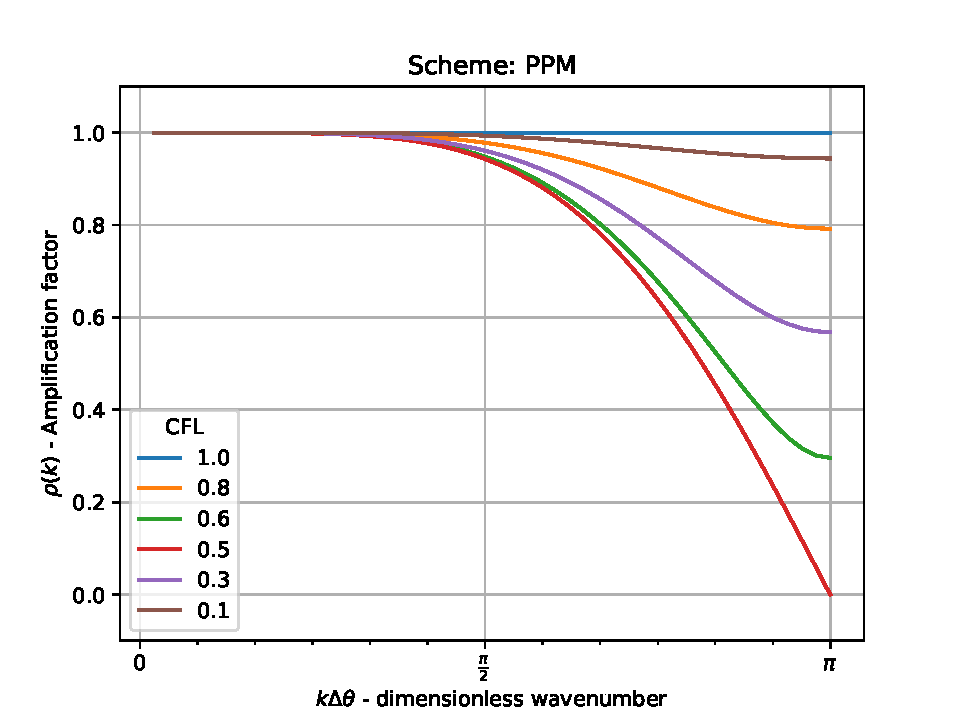
\includegraphics[width=0.49\linewidth]{stability_PPM}
	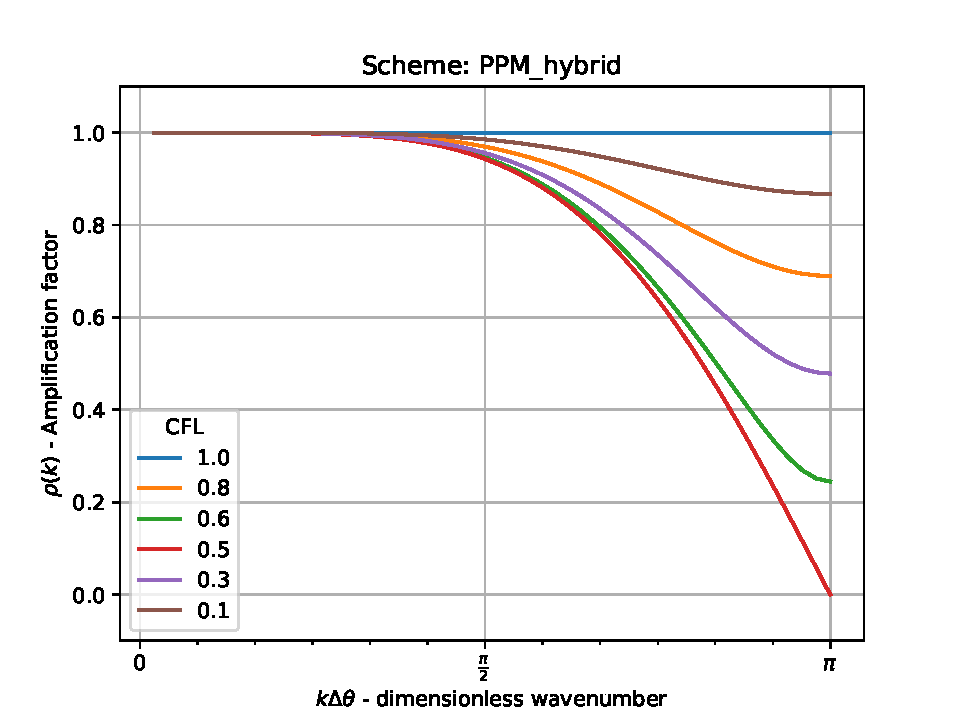
\includegraphics[width=0.49\linewidth]{stability_PPM_hybrid}
	\caption{Amplification factor for the PPM (left) and hybrid PPM (right) schemes for different CFL numbers.}
	\label{chp2-fig-amplification}
\end{figure}
In Figure \ref{chp2-fig-amplification} we show the amplification factor for both PPM and hybrid PPM schemes
considering different CFL numbers.
We can observe that both schemes damp most of the Fourier modes for larger $k$, regardless of the CFL number.
Besides that, the hybrid scheme is more effective when reducing the Fourier modes amplitude.
We point out that both schemes are exact when the CFL number is equal to 1.
From this analysis, we can conclude that the PPM and hybrid PPM schemes satisfy the
Von Neumann stability criteria when the CFL restriction is respected.

In order to investigate the consistency of the PPM scheme, we notice that when we are deducing the time average flux, 
we are making some approximations of the form:
\begin{equation}
	\label{chp2-sec-flux:analysis-eq1}
	\int_{t^n}^{t^{n+1}} (uq)(x_{i+\frac{1}{2}},t) \,dt \approx
  \int_{x_{i+\frac{1}{2}}-u_{i+\frac{1}{2}}^n \Delta t}^{x_{i+\frac{1}{2}}}
	q(x,t^n)\,dx, 
\end{equation}
as we can see from Equations \eqref{chp-sec-flux:fL_1} and \eqref{chp-sec-flux:fR_1},
which basically replace $q$ by $q_{PP}$ on the right-hand side of Equation
\eqref{chp2-sec-flux:analysis-eq1}.
As we shall see, the approximation \eqref{chp2-sec-flux:analysis-eq1}
is in fact exact if we replace $q_{PP}$ by $q$ and assume $u$ does not depend on $x$.
Therefore, in this case, the only error is due to the approximation made by $q_{PP}$. 
In the case when the velocity depends on $x$, these approximations will have two sources
of error: one first-order error in time-related to a computation of a departure point and
another related to the approximation of a time integral by a spatial integral, 
as in \eqref{chp2-sec-flux:analysis-eq1}, which shall be second-order accurate.

For each $s \in [t^n,t^{n+1}]$, let us consider the following Cauchy problem
backward in time:
\begin{equation}
	\label{chp-sec-flux:analysis-eq3}
    	\begin{cases}
				\frac{\partial X}{\partial t} (t,s;x_{i+\frac{1}{2}}) = u(X(t,s;x_{i+\frac{1}{2}}) ,t),\quad t\in[t^{n},s] \\
				X(s,s;x_{i+\frac{1}{2}}) = x_{i+\frac{1}{2}}.
    	\end{cases}
\end{equation}
The point $X(t^n,s;x_{i+\frac{1}{2}})$ is called departure point at time $t^n$
of the point $x_{i+\frac{1}{2}}$ at time $s$.
Integrating Equation $\eqref{chp-sec-flux:analysis-eq3}$ over the interval
$[t,s]$, we get:
\begin{equation}
	\label{chp-sec-flux:analysis-eq4}
	X(t,s;x_{i+\frac{1}{2}}) = x_{i+\frac{1}{2}} - \int_{t}^{s}u(X(\theta,s;x_{i+\frac{1}{2}}),\theta) \,d\theta.
\end{equation}
For instance, if $u$ is constant, then the departure point at time $t^n$ of the point 
$x_{i+\frac{1}{2}}$ at time $t^{n+1}$ is given by:
\begin{equation}
	\label{chp-sec-flux:departurepoint}
	X(t^n,t^{n+1};x_{i+\frac{1}{2}}) = x_{i+\frac{1}{2}} - u\Delta t.
\end{equation}
If the velocity is not constant, it follows from Equation \eqref{chp-sec-flux:analysis-eq4}
that  we can write a second-order approximation to the departure point: 
\begin{equation}
	\label{chp-sec-flux:departurepoint2}
	X(t^n,t^{n+1};x_{i+\frac{1}{2}}) = x_{i+\frac{1}{2}} - u^{n}_{i+\frac{1}{2}}\Delta t + O(\Delta t^2).
\end{equation}
This approximation is exactly what is used in the PPM flux and we give a bound 
to this expression on the next proposition.
\begin{prop}
	Assuming that $u \in C^1$ and $X$ satisfies Equation \eqref{chp-sec-flux:analysis-eq4}, then:
\begin{equation}
	\label{chp-sec-flux:departurepoint3}
	|X(t^n,t^{n+1};x_{i+\frac{1}{2}}) - (x_{i+\frac{1}{2}} - u^{n}_{i+\frac{1}{2}}\Delta t)| \leq M_1 \Delta t^2,
\end{equation}
where $M_1$ is a constant that depends only on $u$. 
\end{prop}
\begin{proof}
	We basically need to estimate the integral of the right-hand side of \eqref{chp-sec-flux:analysis-eq4}.
	Defining $f(t) = u(X(t,t^{n+1};x_{i+\frac{1}{2}}),t)$, it is easy to show that:
	\begin{equation*}
		\bigg|\int_{t^n}^{t^{n+1}}f(t) \,dt - \Delta t f(t^n)\bigg| \leq \frac{\Delta t^2}{2}\sup\{|f'(t)|:t \in [t^n,t^{n+1}]\}
	\end{equation*}
  Writing this expression in terms of $u$, we have:
	\begin{align*}
		\bigg|\int_{t^n}^{t^{n+1}} u(X(t,t^{n+1};x_{i+\frac{1}{2}}),t) \,dt - u^{n}_{i+\frac{1}{2}}\Delta t \bigg|
		&\leq \frac{\Delta t^2}{2}
		\sup_{t \in [t^n,t^{n+1}]} 
		\bigg|\frac{\partial u}{\partial x} 
		(X(t,t^{n+1};x_{i+\frac{1}{2}}),t)
		\frac{\partial X}{\partial t}
		(t,t^{n+1})   
	  +\frac{\partial u}{\partial t} 
		(X(t,t^{n+1};x_{i+\frac{1}{2}}),t)
		\bigg| \\
		& =   
		\frac{\Delta t^2}{2}
		\sup_{t \in [t^n,t^{n+1}]} 
		\bigg|\bigg(\frac{\partial u}{\partial x}u+
		\frac{\partial u}{\partial t}\bigg) 
		(X(t,t^{n+1};x_{i+\frac{1}{2}}),t)
		\bigg| \\ 
		& \leq   
		\frac{\Delta t^2}{2}
		\sup_{t \in [0,T], x \in [a,b]}
		\bigg|\bigg(\frac{\partial u}{\partial x}u+
		\frac{\partial u}{\partial t}\bigg) 
		(x,t)
		\bigg|,
	\end{align*}
	from which the proposition follows with
\begin{equation}
	\label{chp2-sec-flux:M1}
	M_1 =		\frac{1}{2}
		\sup_{t \in [0,T], x \in [a,b]}
		\bigg|\bigg(\frac{\partial u}{\partial x}u+
		\frac{\partial u}{\partial t}\bigg) 
		(x,t)
		\bigg|. 
\end{equation}
\end{proof}
We point out that higher-order departure points estimates may be obtained integrating
the ordinary differential equation \eqref{chp-sec-flux:analysis-eq3} using higher-order time integration schemes.

From Equation \eqref{chp-sec-flux:analysis-eq4}, using the Leibniz rule for integration it follows that:
\begin{align}
	\begin{split}
		\label{chp-sec-flux:dxds}
		\frac{\partial X}{\partial s} (t,s;x_{i+\frac{1}{2}}) &= - \bigg(u(x_{i+\frac{1}{2}},s) + 
		\int_{t}^{s} \frac{du}{ds}(X(\theta,s;x_{i+\frac{1}{2}}),\theta) \,d\theta \bigg)\\
		&=- u(x_{i+\frac{1}{2}},s) -
		\int_{t}^{s} \frac{\partial u}{\partial x}(X(\theta, s; x_{i+\frac{1}{2}}),\theta) 
		\frac{\partial X}{\partial s} (\theta, s; x_{i+\frac{1}{2}})\,d\theta.
	\end{split}
\end{align}
Then, computing $q$ on the trajectory give by $X(t,s;x_{i+\frac{1}{2}})$ and taking
its time derivative, we obtain:
\begin{align}
	\label{chp-sec-flux:dqdt}
	\begin{split}
		\frac{dq}{dt} (X(t,s;x_{i+\frac{1}{2}}),t) &= 
		\frac{\partial q}{\partial t} (X(t,s;x_{i+\frac{1}{2}}),t)+
		u (X(t,s;x_{i+\frac{1}{2}}),t)\frac{\partial q}{\partial x} (X(t,s;x_{i+\frac{1}{2}}),t) \\
		&= -\frac{\partial u}{\partial x}(X(t,s;x_{i+\frac{1}{2}}),t)  q (X(t,s;x_{i+\frac{1}{2}}),t),
	\end{split}
\end{align}
where we used that $q$ satisfies the linear advection equation and that $X(t,s;x_{i+\frac{1}{2}})$
solves Equation \eqref{chp-sec-flux:analysis-eq3}.
Integrating Equation \eqref{chp-sec-flux:dqdt} over $[t,s]$, we have:
\begin{align}
	\begin{split}
		\label{chp-sec-flux:q_int}
		q(X(t,s;x_{i+\frac{1}{2}}),t) &= q(x_{i+\frac{1}{2}},s)
		+ \int_{t}^{s} \frac{\partial u}{\partial x}(X(\theta,s;x_{i+\frac{1}{2}}),\theta) q(X(\theta,s;x_{i+\frac{1}{2}}),\theta) \,d\theta. \\
	\end{split}
\end{align}
Notice that if $u$ does not depend on $x$, then $q$ is constant along the trajectory $X(t,s;x_{i+\frac{1}{2}})$.

Let us consider the mapping $s\in[t^n,t^{n+1}] \to X(t^n,s,x_{i+\frac{1}{2}})$. 
Integrating $q$ over all departure points at time $t^n$ from $x_{i+\frac{1}{2}}$ at time $s$, we have
\begin{equation}
	\label{chp-sec-flux:depint_1}
	-\int^{X(t^n,t^{n};x_{i+\frac{1}{2}}) = x_{i+\frac{1}{2}}}_{X(t^n,t^{n+1};x_{i+\frac{1}{2}})} q(x,t^n)\,dx 
		= \int_{t^n}^{t^{n+1}} q(X(t^n,s;x_{i+\frac{1}{2}}),t^n) \frac{\partial X}{\partial s} (t^n,s;x_{i+\frac{1}{2}})\,ds,
\end{equation}
where we are just using the variable change integration formula.
Then, it follows from Equation \eqref{chp-sec-flux:q_int} with $t=t^n$ that:
\begin{align}
	\label{chp-sec-flux:depint_2}
	\begin{split}
		&-\int_{X(t^n,t^{n+1};x_{i+\frac{1}{2}})}^{x_{i+\frac{1}{2}}} q(x,t^n)\,dx 
		= \int_{t^n}^{t^{n+1}} q(x_{i+\frac{1}{2}},s) \frac{\partial X}{\partial s} (t^n,s;x_{i+\frac{1}{2}}) \,ds \\ 
		+&\int_{t^n}^{t^{n+1}} \int_{t^n}^{s}
		\frac{\partial u}{\partial x}(X(\theta,s;x_{i+\frac{1}{2}}),\theta) q(X(\theta,s;x_{i+\frac{1}{2}}),\theta) 
		\frac{\partial X}{\partial s} (t^n,s;x_{i+\frac{1}{2}}) \,d\theta \,ds.
	\end{split}
\end{align}
Substituting Equation \eqref{chp-sec-flux:dxds} with $t=t^n$ in the first term of the right-hand side
of Equation \eqref{chp-sec-flux:depint_2}, we obtain:
\begin{align}
	\label{chp-sec-flux:depint_3}
	\begin{split}
		&-\int^{x_{i+\frac{1}{2}}}_{X(t^n,t^{n+1};x_{i+\frac{1}{2}})} q(x,t^n)\,dx 
		= -\int_{t^n}^{t^{n+1}} (uq)(x_{i+\frac{1}{2}},s) \,ds \\
		&-\int_{t^n}^{t^{n+1}} \int_{t^n}^{s} \frac{\partial u}{\partial x}(X(\theta,s;x_{i+\frac{1}{2}}),\theta)
		q(x_{i+\frac{1}{2}},s)
		\frac{\partial X}{\partial s} (\theta,s;x_{i+\frac{1}{2}})\,d\theta \,ds\\
		&+ \int_{t^n}^{t^{n+1}} \int_{t^n}^{s}
		\frac{\partial u}{\partial x}(X(\theta,s;x_{i+\frac{1}{2}}),\theta) q(X(\theta,s;x_{i+\frac{1}{2}}),\theta) 
		\frac{\partial X}{\partial s} (t^n,s;x_{i+\frac{1}{2}}) \,d\theta \,ds,\\
	\end{split}
\end{align}
From this we conclude that, if $u$ is constant, then we obtain that the approximation
from Equation and \eqref{chp2-sec-flux:analysis-eq1} is exact.
\begin{prop}
	\label{chp2-sec-flux:prop1}
Assume the framework of Problem \ref{chp2-sec2-prob2}.
If $q$ and $u$ are $\mathcal{C}^1$ functions, then:
\begin{align}
			\label{chp2-sec-flux:approx1}
			\bigg|
			\int_{t^n}^{t^{n+1}} (uq)(x_{i+\frac{1}{2}},s) \,ds -
			\int^{x_{i+\frac{1}{2}}}_{X(t^n,t^{n+1};x_{i+\frac{1}{2}})} q(x,t^n)\,dx 
			\bigg| \leq M_2 \Delta t ^2,
\end{align}
where $M_2$ depends on $q$ and $u$.
\end{prop}

\begin{proof}
Rearranging the terms of \eqref{chp-sec-flux:depint_3}, we obtain:
\begin{align*}
	\label{chp-sec-flux:depint_4}
	\begin{split}
			& \bigg|
			\int_{t^n}^{t^{n+1}} (uq)(x_{i+\frac{1}{2}},s) \,ds -
			\int^{x_{i+\frac{1}{2}}}_{X(t^n,t^{n+1};x_{i+\frac{1}{2}})} q(x,t^n)\,dx 
			\bigg| \leq \\
			& \int_{t^n}^{t^{n+1}} \int_{t^n}^{s} \bigg| 
			\frac{\partial u}{\partial x}(X(\theta,s;x_{i+\frac{1}{2}}),t) \bigg(q(x_{i+\frac{1}{2}},s)
			\frac{\partial X}{\partial s} (\theta,s;x_{i+\frac{1}{2}})- 
			q(X(\theta,s;x_{i+\frac{1}{2}}),\theta) 
			\frac{\partial X}{\partial s} (t^n,s;x_{i+\frac{1}{2}})\bigg)\bigg| \,d\theta \,ds \leq\\
			& 2M_2 \int_{t^n}^{t^{n+1}} \int_{t^n}^{s}  \,d\theta \,ds \leq M_2 \Delta t ^2,
	\end{split}
\end{align*}
where
\begin{equation}
	\label{chp2-sec-flux:M2}
	M_2 = \frac{1}{2} 
			\sup_{t\in[0,T], x\in[a,b]}\bigg| 
			\frac{\partial u}{\partial x}(x,t) 
			q(x,t) \bigg(
			\frac{\partial X}{\partial s} (\theta,s;x_{i+\frac{1}{2}})+
			\frac{\partial X}{\partial s} (t^n,s;x_{i+\frac{1}{2}})\bigg)\bigg|.
\end{equation}
\end{proof}
\begin{remark}
	If $u$ does not depend on $x$, then $M_2=0$ and the formula given in Equation 
	\eqref{chp2-sec-flux:M1} is exact.
\end{remark}
The next proposition gives an estimate to the approximation \eqref{chp2-sec-flux:analysis-eq1},
where we are going to use an estimate to compute the departure point in Equation \eqref{chp2-sec-flux:approx1}.
\begin{prop}
	Under the same assumptions of Proposition \eqref{chp2-sec-flux:prop1}, we have:
	\begin{equation}
	\bigg|
			  \int_{t^n}^{t^{n+1}} (uq)(x_{i+\frac{1}{2}},s) \,ds 
			 -\int^{x_{i+\frac{1}{2}}}_{x_{i+\frac{1}{2}}-u_i^n \Delta t} q(x,t^n)\,dx
	\bigg| \leq M_3 \Delta t^2, 
	\end{equation}
	where $M_3$ depends on $q$ and $u$.
\end{prop}
\begin{proof}
	Using Equations \eqref{chp-sec-flux:departurepoint3} and \eqref{chp2-sec-flux:approx1}, we get: 
	\begin{align*}
	\label{chp-sec-flux:depint_5}
			 &\bigg|
			  \int_{t^n}^{t^{n+1}} (uq)(x_{i+\frac{1}{2}},s) \,ds 
			 -\int^{x_{i+\frac{1}{2}}}_{x_{i+\frac{1}{2}}-u_{i+\frac{1}{2}}^n \Delta t} q(x,t^n)\,dx
			 \bigg|=
			 \\
			 &\bigg|
			  \int_{t^n}^{t^{n+1}} (uq)(x_{i+\frac{1}{2}},s) \,ds  
			 -\int^{x_{i+\frac{1}{2}}}_{X(t^n,t^{n+1};x_{i+\frac{1}{2}})} q(x,t^n)\,dx \bigg|
			 +\bigg|\int^{x_{i+\frac{1}{2}}}_{X(t^n,t^{n+1};x_{i+\frac{1}{2}})} q(x,t^n)\,dx
			 -\int^{x_{i+\frac{1}{2}}}_{x_{i+\frac{1}{2}}-u_{i+\frac{1}{2}}^n \Delta t} q(x,t^n)\,dx 
			 \bigg| \leq
			 \\
			 &M_2 \Delta t^2+ 
			 \bigg|\int_{X(t^n,t^{n+1};x_{i+\frac{1}{2}})}^{x_{i+\frac{1}{2}}-u_{i+\frac{1}{2}}^n \Delta t} q(x,t^n)\,dx 
			 \bigg| \leq M \Delta t^2 + 
			 \big|X(t^n,t^{n+1};x_{i+\frac{1}{2}}) - x_{i+\frac{1}{2}}-u_{i+\frac{1}{2}}^n \Delta t \big|
			 \sup_{x\in[a,b], t\in[0,T]} {|q(x,t)|} \\
			  &\leq  M_1 \Delta t^2 \sup_{x\in[a,b], t\in[0,T]}{|q(x,t)|} + M_2 \Delta t^2 \leq M_3 \Delta t ^2,
\end{align*}
	with
	\begin{equation}
		\label{chp2-sec-flux-M3}
		M_3 = M_1 \sup_{x\in[a,b], t\in[0,T]}{|q(x,t)|} + M_2, 
	\end{equation}
	where $M_1$ is given by \eqref{chp2-sec-flux:M1}
	and $M_2$ is given by \eqref{chp2-sec-flux:M2}.
\end{proof}
Thus, in the PPM flux estimation, we have a first-order error related to the departure point
computation and a second-order error related to the approximation of a temporal integral using
a spatial integral. We point out that, if the velocity is constant, then no error is obtained
using the PPM flux, except for the approximation $q_{PP}$ to $q$.
\begin{prop}
	Assuming the CFL condition, and denote by $q_{PP}$ the Piecewise-Parabolic approximation of $q(x,t^n)$.
	Under the same assumptions of Proposition \eqref{chp2-sec-flux:prop1}, we have:
	\begin{equation}
		\bigg| \frac{1}{\Delta t}\int_{t^n}^{t^{n+1}} (uq)(x_{i+\frac{1}{2}},s) \,ds - 
		\mathcal{F}(Q(t_n);u^n;i)  \bigg| \leq \Delta t + M_4\Delta x^3,
	\end{equation}
	where $M_4$ are constants depending only on $q$ and $u$.
\end{prop}
\begin{proof}
	By Proposition \ref{prop:ppm-bound4} we have $|q(x,t^n)-q_{i}(x)| \leq M_4 \Delta x^4$,
	$\forall x \in X_i$, where $M_4$ depends only on $q$. Besides that,
	\begin{align*}
	 &\bigg|
	 \frac{1}{\Delta t}\int_{t^n}^{t^{n+1}} (uq)(x_{i+\frac{1}{2}},s) \,ds - 
	\mathcal{F}(Q(t_n);u^n;i)  \bigg| =
	 \bigg|
	 \frac{1}{\Delta t}\int_{t^n}^{t^{n+1}} (uq)(x_{i+\frac{1}{2}},s) \,ds - 
	 \frac{1}{\Delta t}\int^{x_{i+\frac{1}{2}}}_{x_{i+\frac{1}{2}}-u_{i+\frac{1}{2}}^n \Delta t} q_{PP}(x)\,dx  \bigg| =
	 \\
	 &\frac{1}{\Delta t}\bigg|
	 \int_{t^n}^{t^{n+1}} (uq)(x_{i+\frac{1}{2}},s) \,ds 
	 -\int^{x_{i+\frac{1}{2}}}_{x_{i+\frac{1}{2}}-u_{i+\frac{1}{2}}^n \Delta t} q_{i}(x)\,dx \bigg| \leq
	 \\
	 &\frac{1}{\Delta t}\bigg|
			\int_{t^n}^{t^{n+1}} (uq)(x_{i+\frac{1}{2}},s) \,ds 
			-\int^{x_{i+\frac{1}{2}}}_{x_{i+\frac{1}{2}}-u_{i+\frac{1}{2}}^n \Delta t} q(x,t^n)\,dx\bigg| 
			+\frac{1}{\Delta t}\bigg|\int^{x_{i+\frac{1}{2}}}_{x_{i+\frac{1}{2}}-u_{i+\frac{1}{2}}^n \Delta t} q(x,t^n)\,dx 
			-\int^{x_{i+\frac{1}{2}}}_{x_{i+\frac{1}{2}}-u_{i+\frac{1}{2}}^n \Delta t} q_{i}(x)\,dx 
		  \bigg| \leq \\
			& M_3\Delta t + 
			\int^{x_{i+\frac{1}{2}}}_{x_{i+\frac{1}{2}}-u_{i+\frac{1}{2}}^n \Delta t} |q(x,t^n)-q_{i}(x)|\,dx
			\leq M_3 \Delta t +  M_4 \Delta x^3
\end{align*}
\end{proof}
where $M_3$ is given by Equation \eqref{chp2-sec-flux-M3}.

\newpage
\section{Numerical experiements}
\label{chp2-sec-numerical-exp}
This Section is dedicated to presenting the numerical results of the PPM and its variations discussed here.
For non-monotonic schemes, we are going to consider
the original PPM from \citet{colella:1984} and the hybrid PPM from \citet{putman:2007}.
For monotonic schemes, we are going to consider the monotonization schemes from 
\citet{colella:1984} and \citet{lin:2004}, which are referred to as CW84 monotonization 
and L04 monotonization hereafter.
In Subsection \ref{chp2-sec-numerical-exp-1} we present results 
using the linear advection equation with constant velocity
and in Subsection \ref{chp2-sec-numerical-exp-2}
the results are based on the linear advection equation with variable velocity.
The code used in this Section may be found in Appendix \ref{anexo-code}.

\subsection{Linear advection equation with constant velocity simulations}
\label{chp2-sec-numerical-exp-1}

For the linear advection equation with the constant velocity we shall adopt the $u=0.2$ and 
a CFL number equal to $0.8$.
The spatial domain will be given by $[0,1]$ and the time integration interval will be $[0,5]$.
Since we are going to assume periodic boundary conditions, the period is equal to $5$. 
Hence, the simulations presented here shall advect an initial profile for one time period. 
This shall be the general setup for all simulations presented in this subsection. 
What will distinguish the simulations is the initial condition.
The first $q_0$ is given by:
\begin{equation}
	\label{chp2-ic1}
	q_0(x) = \sin (2\pi k x) + 1.
\end{equation}
Here $k$ denotes the wavenumber and we adopt $k=5$.
Inspired by \citet{trefethen:2000}, we adopted the following periodic Gaussian profile.
\begin{equation}
	\label{chp2-ic2}
		q_0(x) = \exp(-10\cos^2 (2\pi x)).
\end{equation}
Both functions from Equations \eqref{chp2-ic2} and \eqref{chp2-ic2} are smooth.
We also consider a discontinuous initial condition given by:
\begin{equation}
	\label{chp2-ic3}
		q_0(x) =  
  \begin{cases}
		1 & \text{if } x \in [0.4,0.6],\\
		0 & \text{otherwise}.
  \end{cases}
\end{equation}
It is easy to check that the  exact solution of Problem \ref{chp2-sec2-prob1}
is given by $q_0(x-ut)$ for all $q_0$ presented here.

As pointed in Subsection \ref{chp2-sub-CC}, when $q_0$ is given by Equation \eqref{chp2-ic2},
we are going to compute the initial average values $Q_i(0)$ using
the initial values of $q^0_i$ at the control volume centroids, which is second-order 
accurate by Proposition \ref{prop-bound-centroid}.
In the error calculation, only when $q_0$ is given by Equation \eqref{chp2-ic2},
we replace $Q_{i}(t^n)$ by its centroid value $q_{i}(t^n)$, which again gives
a second-order approximation by Proposition \ref{prop-bound-centroid}.
Therefore, since $q_0$ is smooth, we expect that the error convergence shall be at least second-order accurate.
Finally, the error norm is normalized by dividing the error norm by the exact solution norm. 
The norm adopted here is the maximum norm.

\newpage
\begin{figure}[!htb]
  \centering
  \begin{subfigure}{0.45\textwidth}
    \centering
			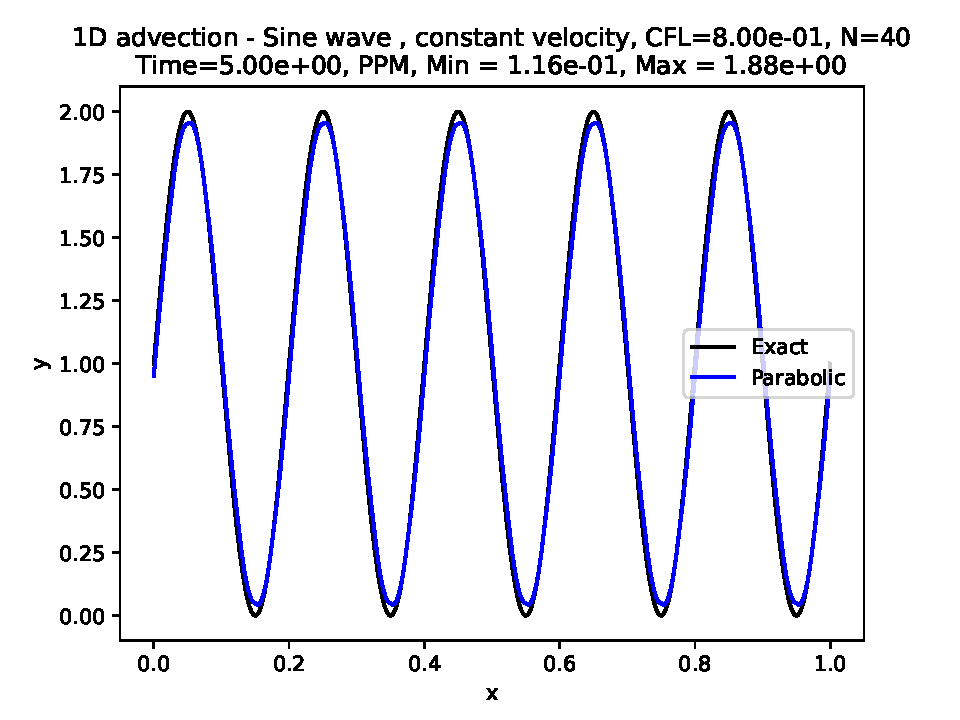
\includegraphics[width=1\linewidth]{1d_adv_tc2_ic1_vf1_t49_N40_PPM}
			\caption{PPM.\label{chp2-sec-exp-adv1-a}}
  \end{subfigure}
  \begin{subfigure}{0.45\textwidth}
    \centering
			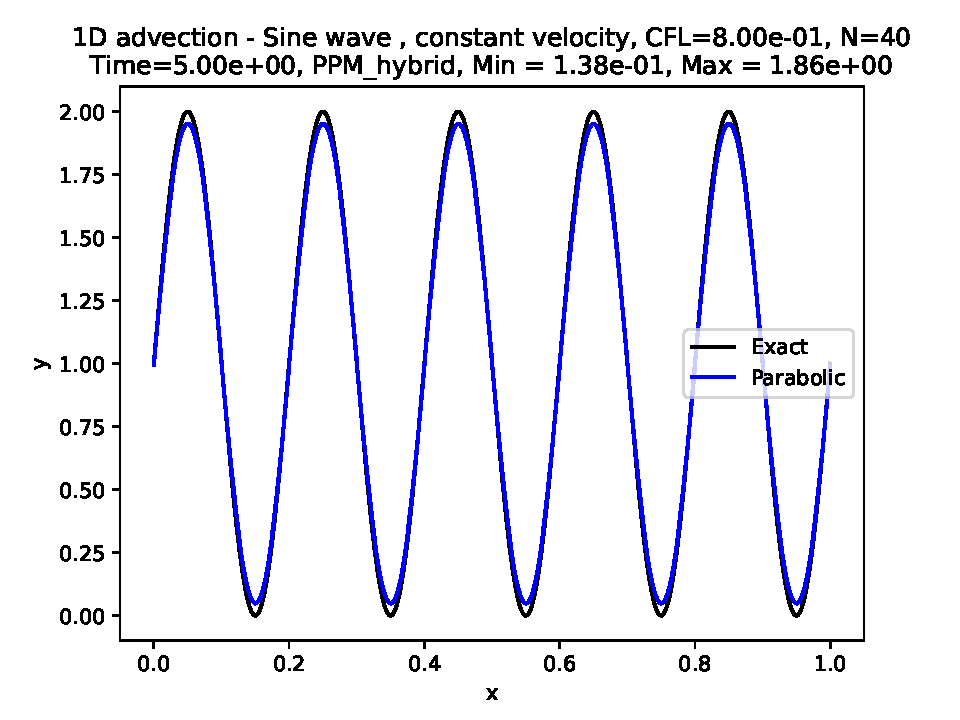
\includegraphics[width=1\linewidth]{1d_adv_tc2_ic1_vf1_t49_N40_PPM_hybrid}
			\caption{Hybrid PPM.\label{chp2-sec-exp-adv1-b}}
  \end{subfigure}

  \begin{subfigure}{0.45\textwidth}
    \centering
		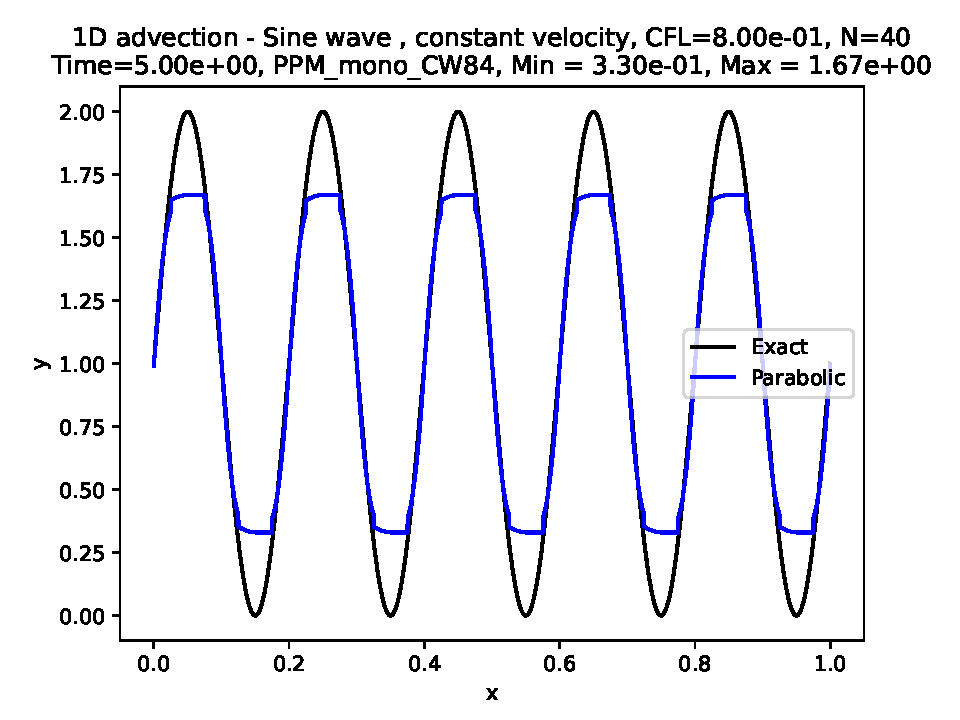
\includegraphics[width=1\linewidth]{1d_adv_tc2_ic1_vf1_t49_N40_PPM_mono_CW84}
    \caption{PPM + CW84 monotonization.\label{chp2-sec-exp-adv1-c}}
  \end{subfigure}
  \begin{subfigure}{0.45\textwidth}
    \centering
			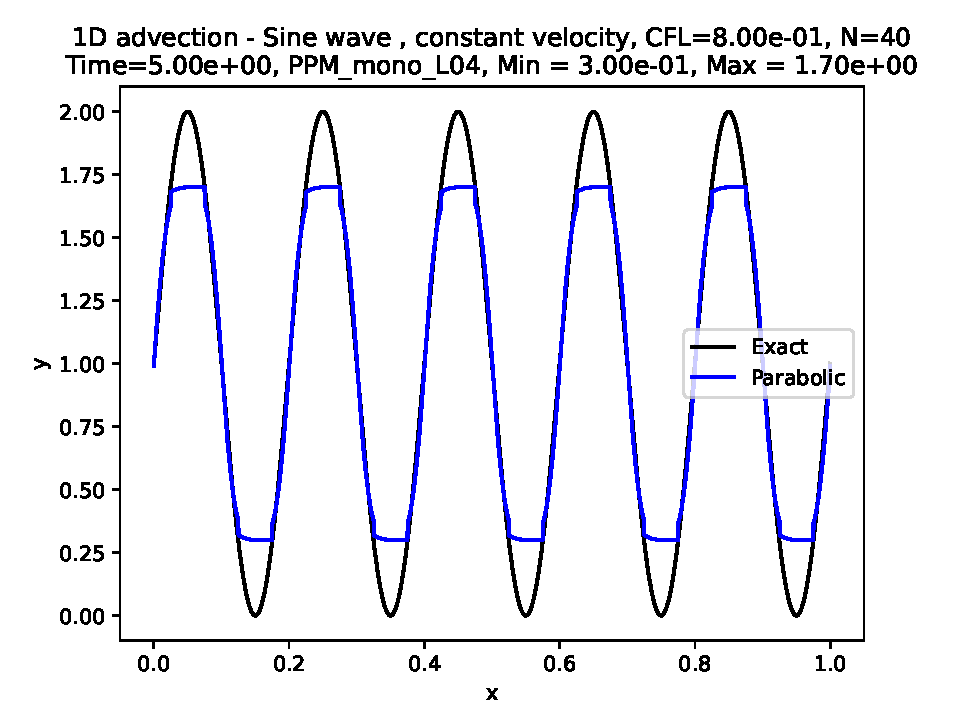
\includegraphics[width=1\linewidth]{1d_adv_tc2_ic1_vf1_t49_N40_PPM_mono_L04}
      \caption{PPM + L04 monotonization.\label{chp2-sec-exp-adv1-d}}
  \end{subfigure} 
	\caption{Linear advection experiement using a constant velocity equal to $0.1$,
  a CFL number equal to $0.8$, $N=40$ cells, and the initial condition is given by Equation \eqref{chp2-ic1}.
	These figures show the advected profile after 5 seconds (one time period).
	Schemes employed: PPM (a), hybrid PPM (b), PPM with the CW84 monotonization
	(c) and PPM with L04 monotonization (d). \label{chp2-sec-exp-adv1}}
\end{figure}

\begin{figure}[!htb]
  \centering
  \begin{subfigure}{0.45\textwidth}
    \centering
		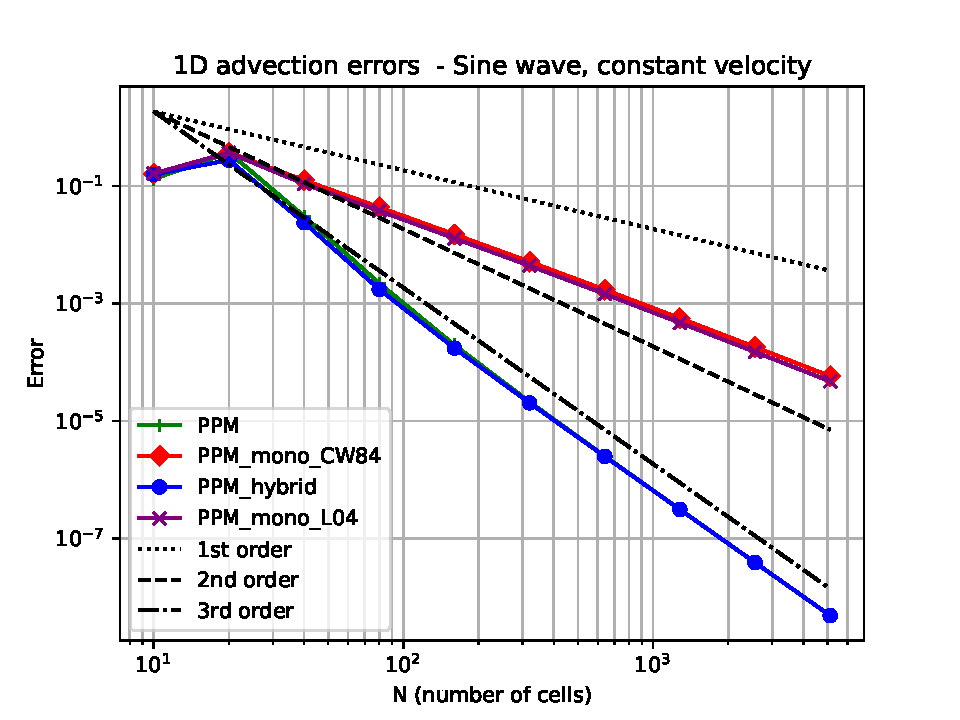
\includegraphics[width=1\linewidth]{1d_adv_tc2_ic1_vf1_parabola_errors}
		\caption{Error.\label{chp2-sec-exp-adv1-error}}
  \end{subfigure}
  \begin{subfigure}{0.45\textwidth}
    \centering
			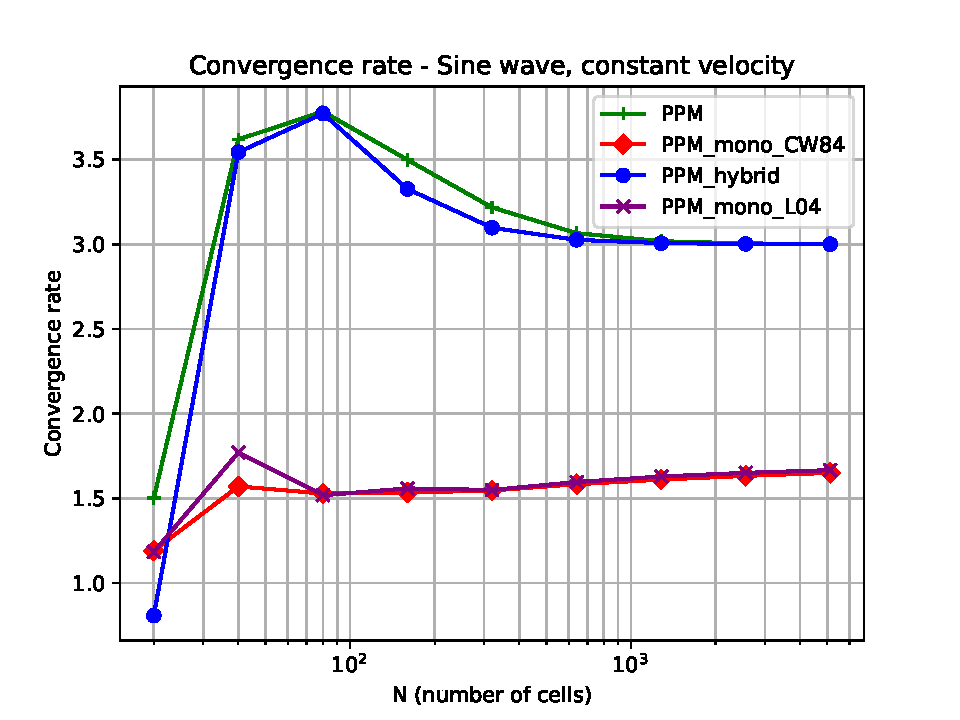
\includegraphics[width=1\linewidth]{1d_adv_tc2_ic1_vf1_convergence_rate}
		\caption{Convergence rate.\label{chp2-sec-exp-adv1-CR}}
  \end{subfigure}
	\caption{Convergence of the error (a) and convergence rate (b) for the schemes
  PPM, hybrid PPM, PPM with the CW84 monotonization and PPM with L04 monotonization
	applied to the linear advection problem using a constant velocity equal to $0.1$,
	a CFL number equal to $0.8$, a final time of integration equal to 5 seconds
	and the initial condition given by Equation \eqref{chp2-ic1}.\label{chp2-sec-exp-adv1-2}}
\end{figure}

\newpage

\begin{figure}[!htb]
  \centering
  \begin{subfigure}{0.49\textwidth}
    \centering
			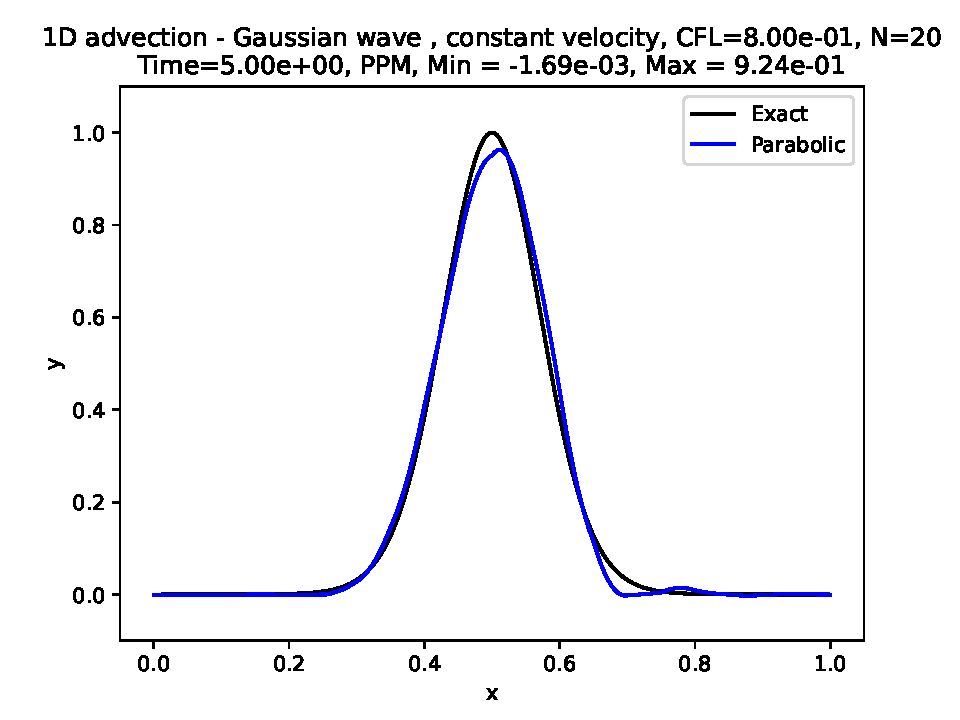
\includegraphics[width=1\linewidth]{1d_adv_tc2_ic2_vf1_t24_N20_PPM}
			\caption{PPM.\label{chp2-sec-exp-adv2-a}}
  \end{subfigure}
  \begin{subfigure}{0.49\textwidth}
    \centering
			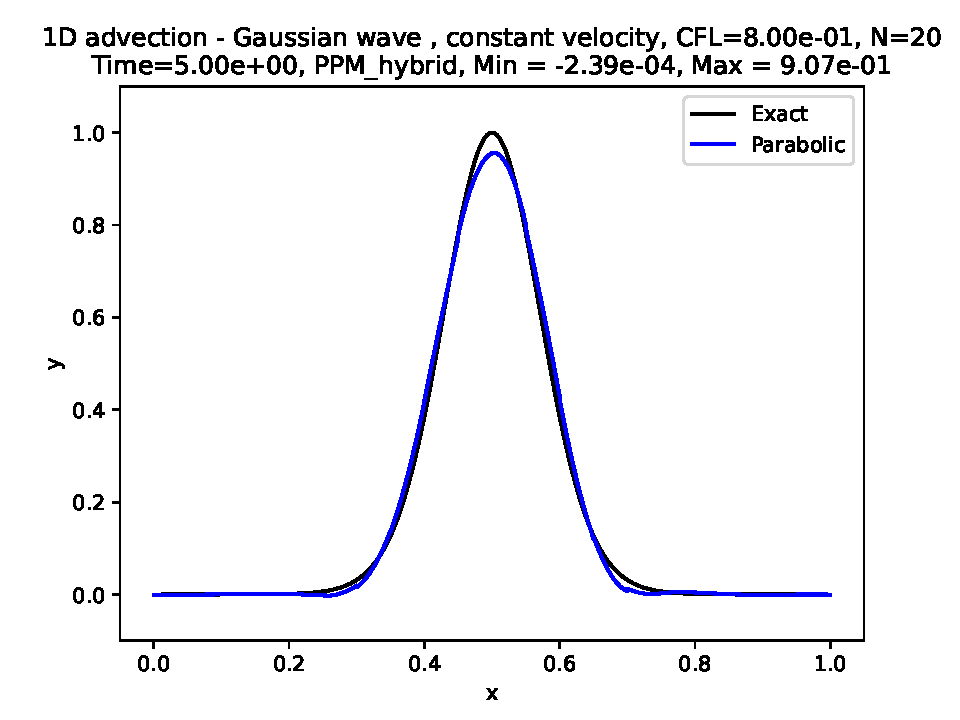
\includegraphics[width=1\linewidth]{1d_adv_tc2_ic2_vf1_t24_N20_PPM_hybrid}
			\caption{Hybrid PPM.\label{chp2-sec-exp-adv2-b}}
  \end{subfigure}

  \begin{subfigure}{0.49\textwidth}
    \centering
		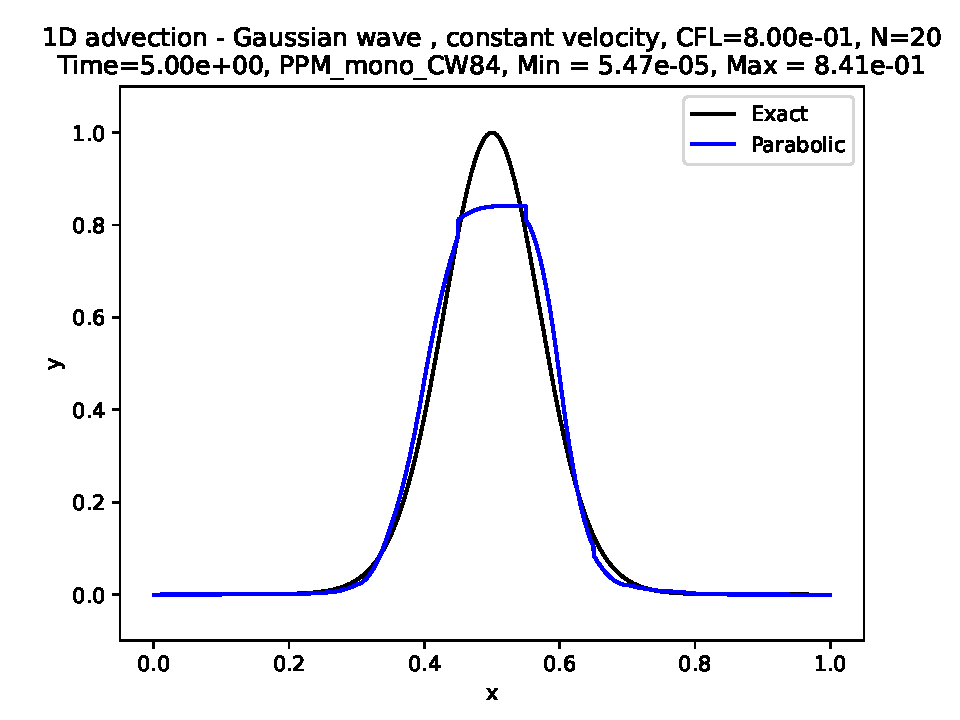
\includegraphics[width=1\linewidth]{1d_adv_tc2_ic2_vf1_t24_N20_PPM_mono_CW84}
    \caption{PPM + CW84 monotonization.\label{chp2-sec-exp-adv2-c}}
  \end{subfigure}
  \begin{subfigure}{0.49\textwidth}
    \centering
			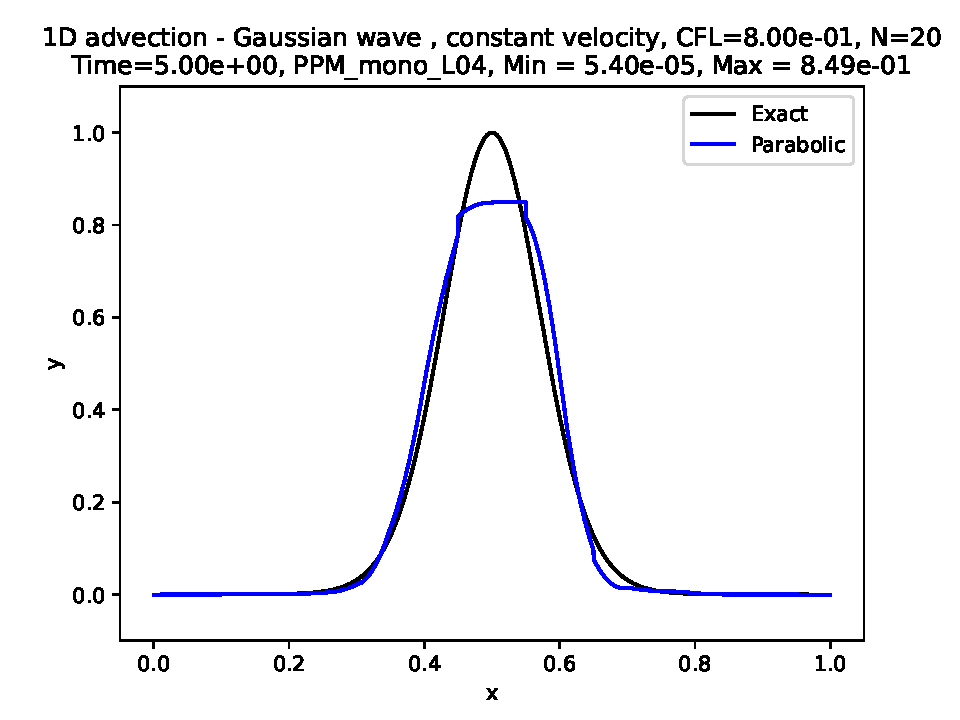
\includegraphics[width=1\linewidth]{1d_adv_tc2_ic2_vf1_t24_N20_PPM_mono_L04}
      \caption{PPM + L04 monotonization.\label{chp2-sec-exp-adv2-d}}
  \end{subfigure} 
	\caption{ Similar to Figure \ref{chp2-sec-exp-adv1} but using $N=20$
	and the initial condition given by Equation \eqref{chp2-ic2}.\label{chp2-sec-exp-adv2}}
\end{figure}

\begin{figure}[!htb]
  \centering
  \begin{subfigure}{0.49\textwidth}
    \centering
		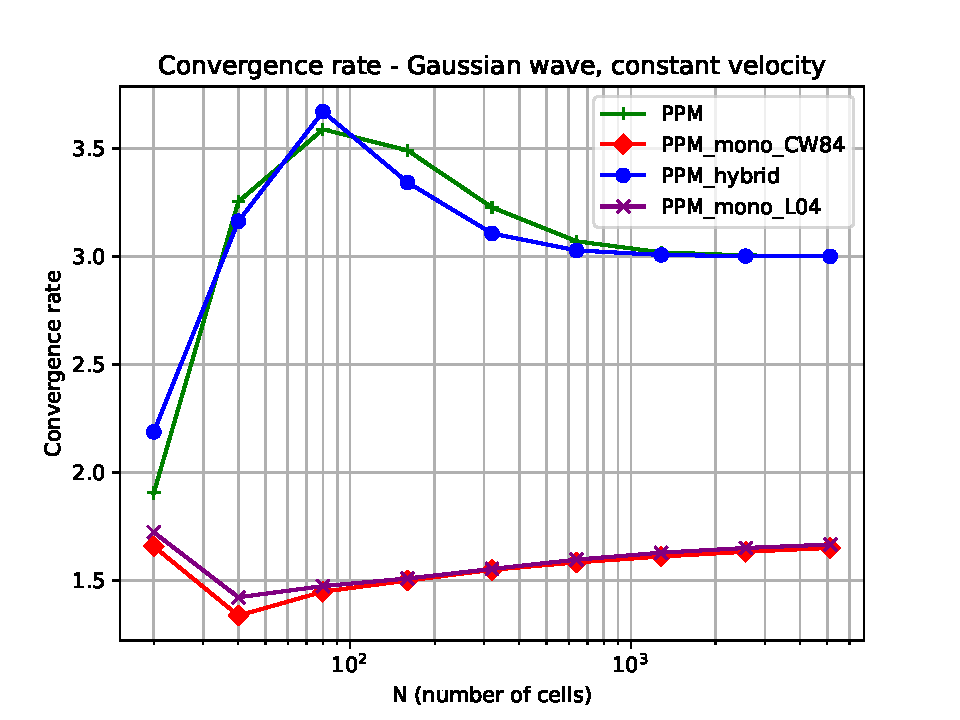
\includegraphics[width=1\linewidth]{1d_adv_tc2_ic2_vf1_convergence_rate}
		\caption{Error.\label{chp2-sec-exp-adv2-error}}
  \end{subfigure}
  \begin{subfigure}{0.49\textwidth}
    \centering
			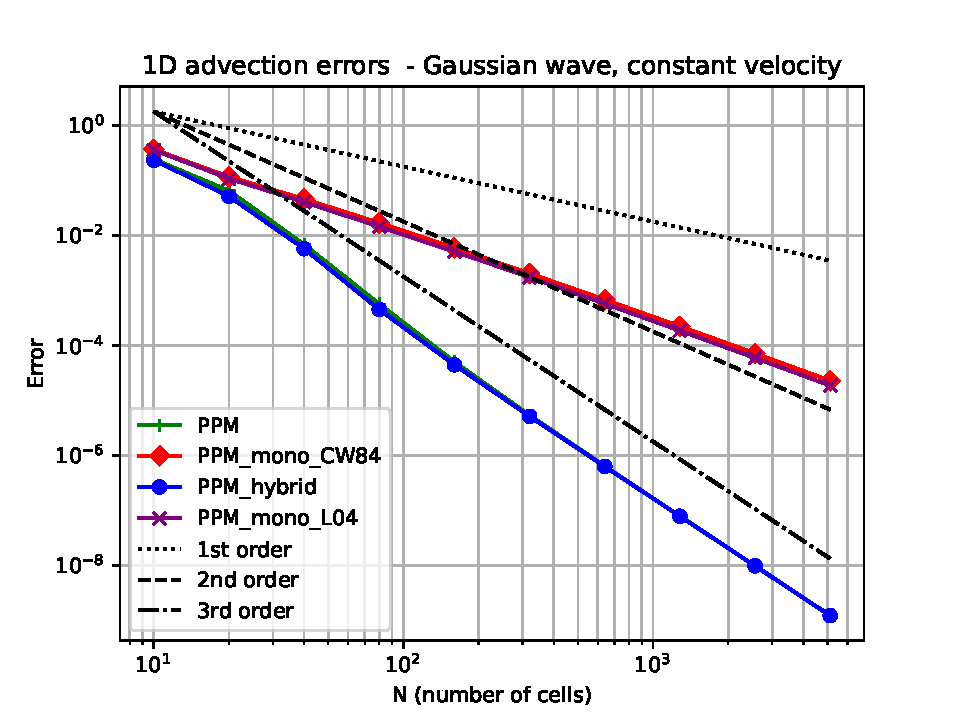
\includegraphics[width=1\linewidth]{1d_adv_tc2_ic2_vf1_parabola_errors}
		\caption{Convergence rate.\label{chp2-sec-exp-adv2-CR}}
  \end{subfigure}
	\caption{ Similar to Figure \ref{chp2-sec-exp-adv1-2} but using
	the initial condition given by Equation \eqref{chp2-ic2}. \label{chp2-sec-exp-adv2-2}}
\end{figure}

\newpage

\begin{figure}[!htb]
  \centering
  \begin{subfigure}{0.49\textwidth}
    \centering
			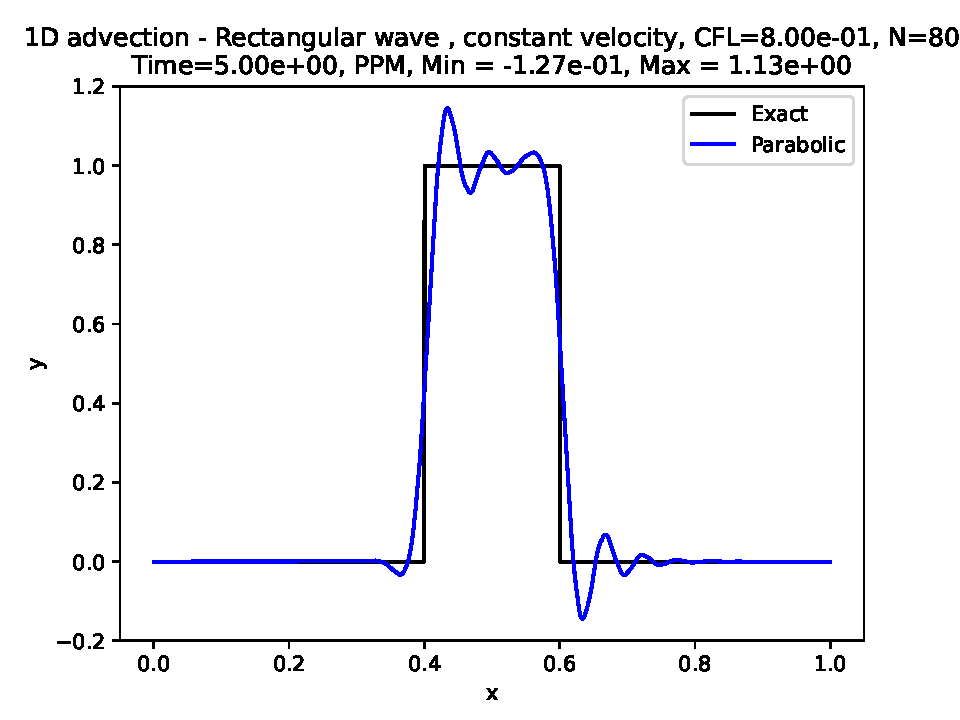
\includegraphics[width=1\linewidth]{1d_adv_tc2_ic4_vf1_t99_N80_PPM}
			\caption{PPM.\label{chp2-sec-exp-adv3-a}}
  \end{subfigure}
  \begin{subfigure}{0.49\textwidth}
    \centering
			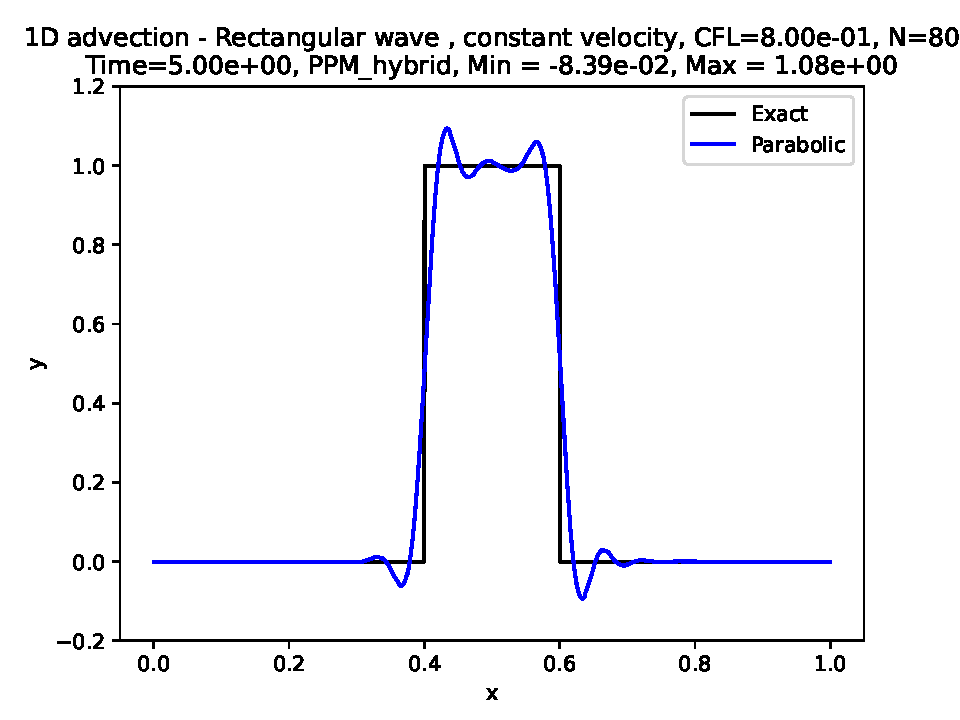
\includegraphics[width=1\linewidth]{1d_adv_tc2_ic4_vf1_t99_N80_PPM_hybrid}
			\caption{Hybrid PPM.\label{chp2-sec-exp-adv3-b}}
  \end{subfigure}

  \begin{subfigure}{0.49\textwidth}
    \centering
		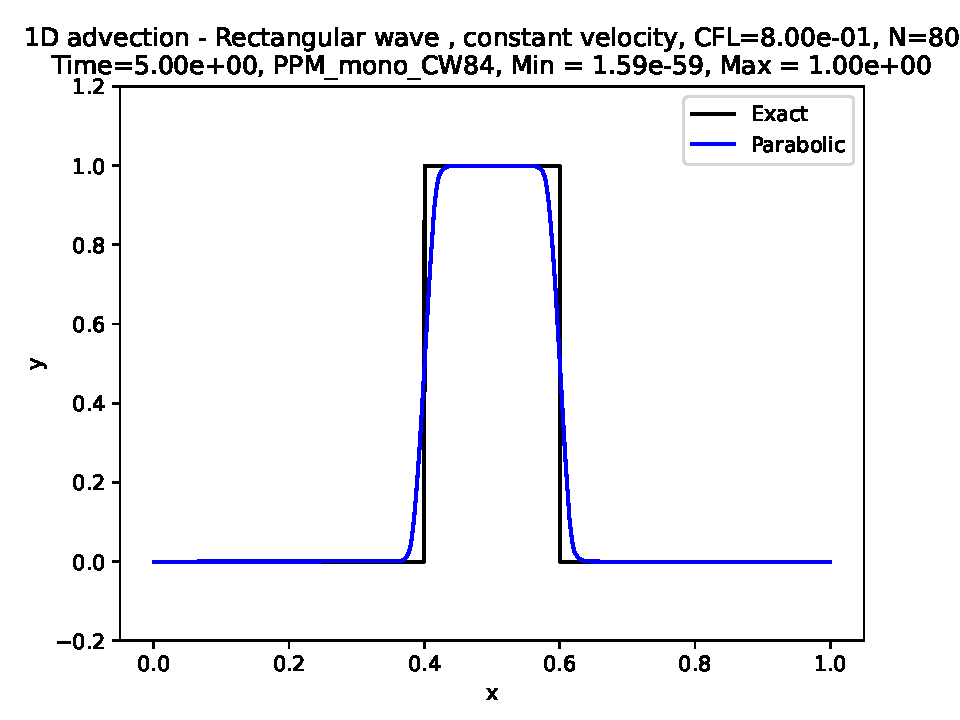
\includegraphics[width=1\linewidth]{1d_adv_tc2_ic4_vf1_t99_N80_PPM_mono_CW84}
    \caption{PPM + CW84 monotonization.\label{chp2-sec-exp-adv3-c}}
  \end{subfigure}
  \begin{subfigure}{0.49\textwidth}
    \centering
			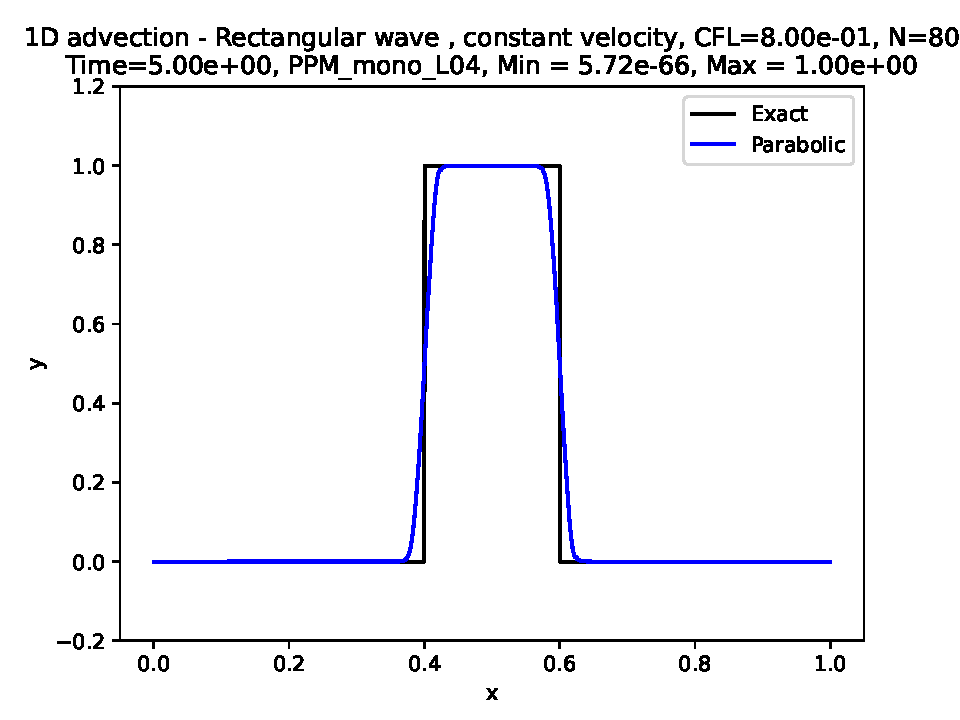
\includegraphics[width=1\linewidth]{1d_adv_tc2_ic4_vf1_t99_N80_PPM_mono_L04}
      \caption{PPM + L04 monotonization.\label{chp2-sec-exp-adv3-d}}
  \end{subfigure} 
	\caption{ Similar to Figure \ref{chp2-sec-exp-adv1} but using $N=80$
	and the initial condition given by Equation \eqref{chp2-ic3}.\label{chp2-sec-exp-adv3}}
\end{figure}
OKOK

\newpage

\subsection{Linear advection equation with variable velocity simulations}
\label{chp2-sec-numerical-exp-2}

In this Subsection, we shall investigate the how the PPM schemes behaves when the velocity is variable.
The initial condition is always given by Equation \eqref{chp2-ic2}.
The relative errors are computed using the centroid values of $q$ as described in
Subsection \ref{chp2-sec-numerical-exp-2}. We are going to consider the velocities
\begin{equation}
	\label{chp2-vel1}
	u(x,t) = u_0\cos{\bigg(\frac{\pi t}{T}\bigg)},
\end{equation}
and
\begin{equation}
	\label{chp2-vel2}
	u(x,t) = u_0\cos{\bigg(\frac{\pi t}{T}\bigg)}\sin^2(\pi x).
\end{equation}
We adopt the parameters $u_0 = 0.2$ and $T = 5$.
In both cases, the solution has a period equal to 5.
Therefore, the profile after 5 seconds is equal to the initial profile and we can compute the error.
We remark that the velocity from Equation \eqref{chp2-vel2} is based on the deformational flow 
test case from on\citet{nair:2010}.

The velocity from Equation \eqref{chp2-vel1} varies only with time 
while the velocity from Equation \eqref{chp2-vel2} varies with both time and space.
\newpage

\begin{figure}[!htb]
  \centering
  \begin{subfigure}{0.49\textwidth}
    \centering
			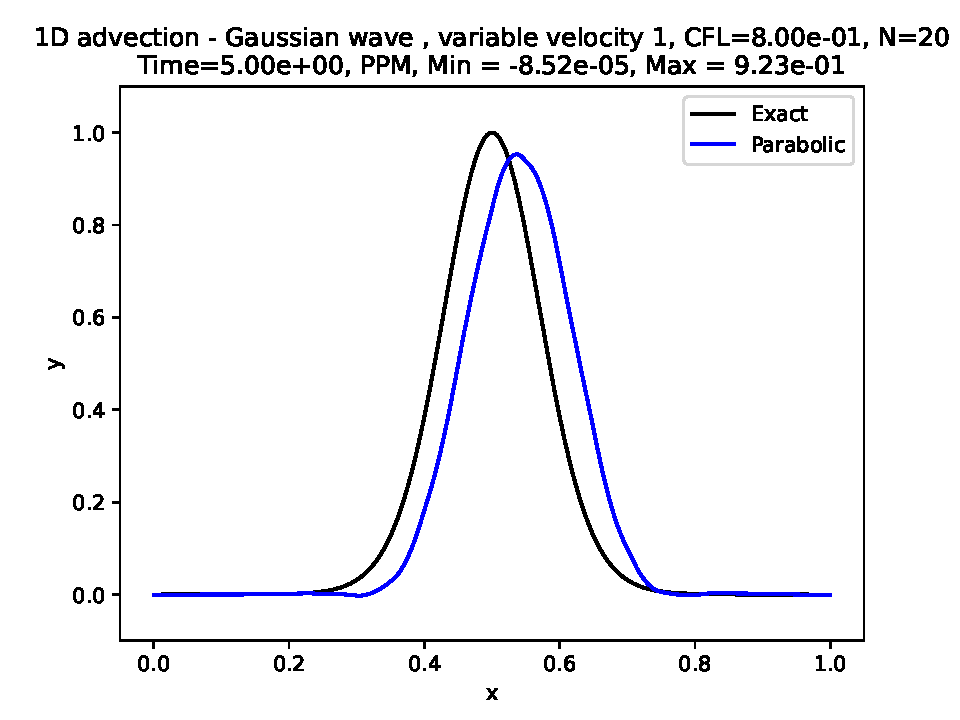
\includegraphics[width=1\linewidth]{1d_adv_tc2_ic2_vf2_t24_N20_PPM}
			\caption{PPM.\label{chp2-sec-exp-adv4-a}}
  \end{subfigure}
  \begin{subfigure}{0.49\textwidth}
    \centering
			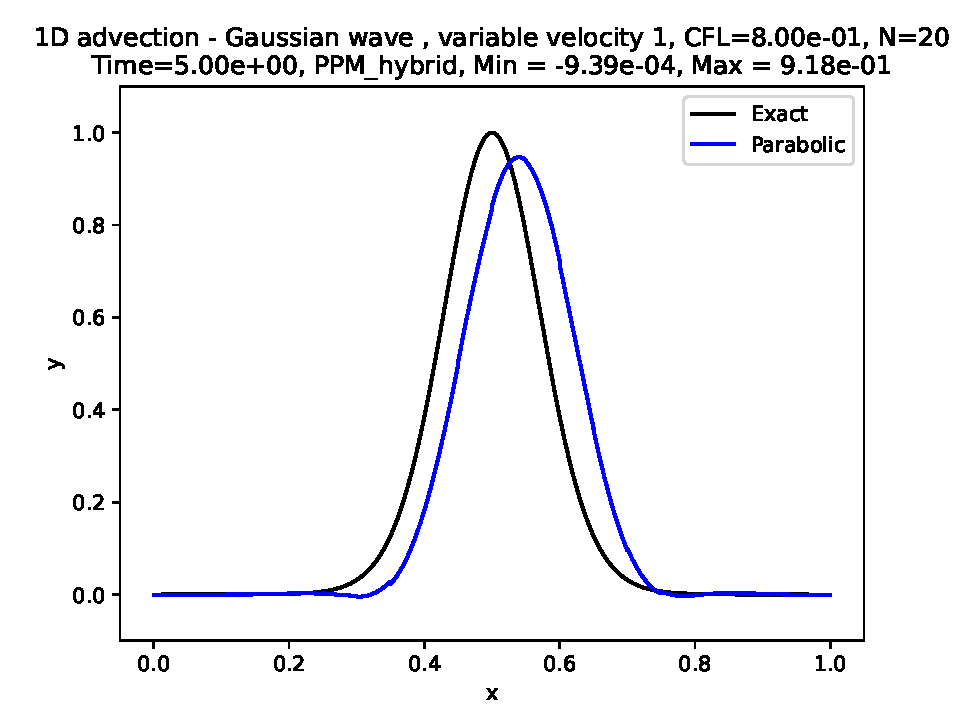
\includegraphics[width=1\linewidth]{1d_adv_tc2_ic2_vf2_t24_N20_PPM_hybrid}
			\caption{Hybrid PPM.\label{chp2-sec-exp-adv4-b}}
  \end{subfigure}

  \begin{subfigure}{0.49\textwidth}
    \centering
		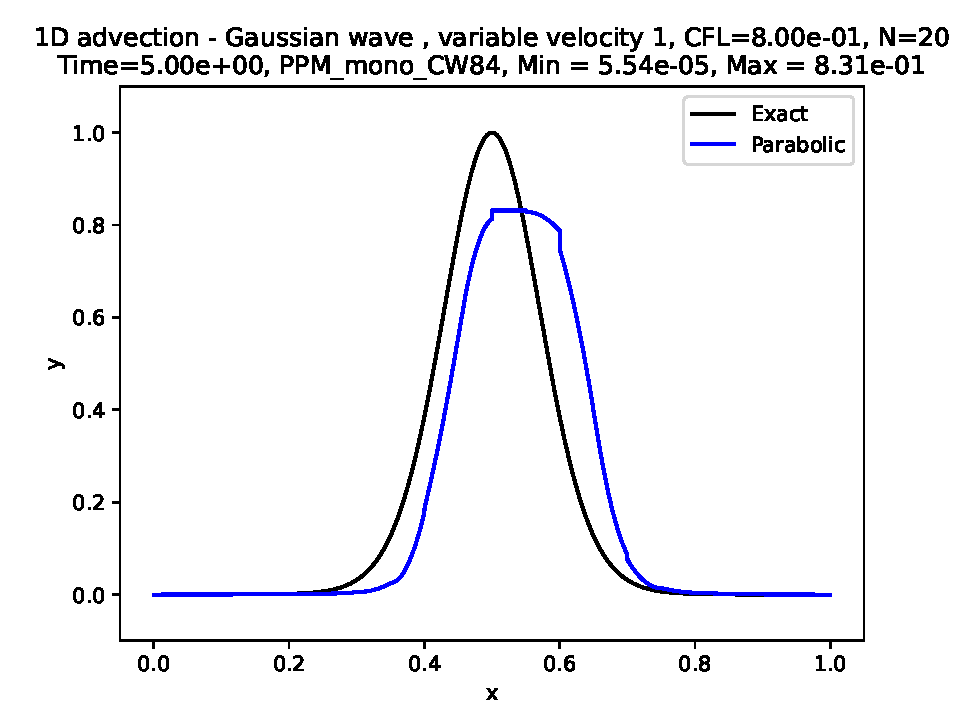
\includegraphics[width=1\linewidth]{1d_adv_tc2_ic2_vf2_t24_N20_PPM_mono_CW84}
    \caption{PPM + CW84 monotonization.\label{chp2-sec-exp-adv4-c}}
  \end{subfigure}
  \begin{subfigure}{0.49\textwidth}
    \centering
			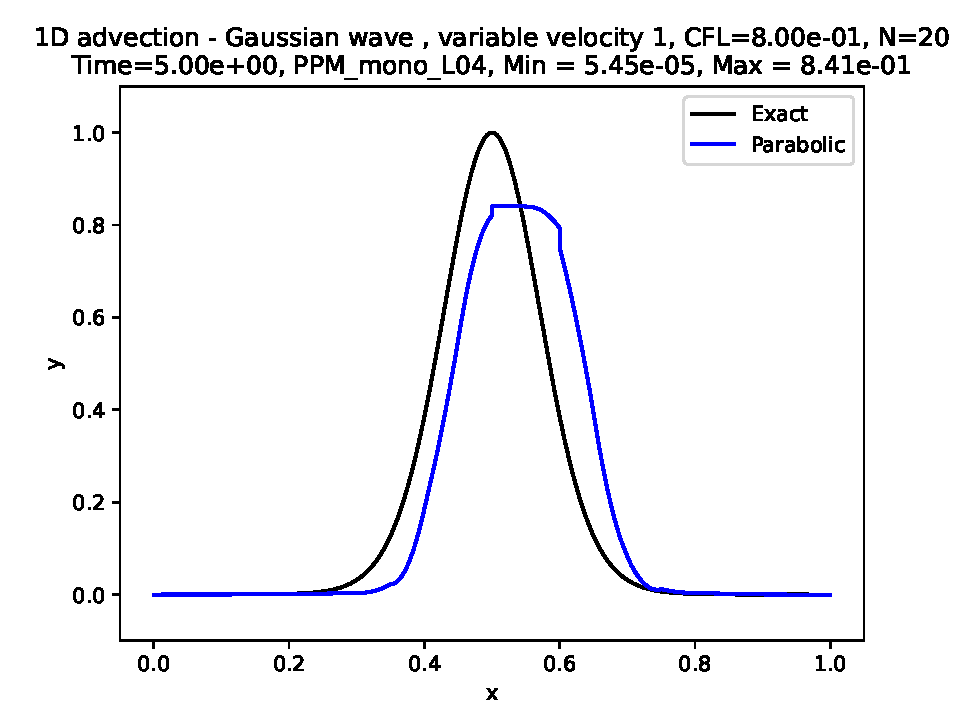
\includegraphics[width=1\linewidth]{1d_adv_tc2_ic2_vf2_t24_N20_PPM_mono_L04}
      \caption{PPM + L04 monotonization.\label{chp2-sec-exp-adv4-d}}
  \end{subfigure} 
	\caption{ Similar to Figure \ref{chp2-sec-exp-adv1} but using $N=20$, the initial
	condition given by Equation \eqref{chp2-ic2} and the variable velocity given by Equation 
	\label{chp2-sec-exp-adv4}}
\end{figure}

\begin{figure}[!htb]
  \centering
  \begin{subfigure}{0.49\textwidth}
    \centering
		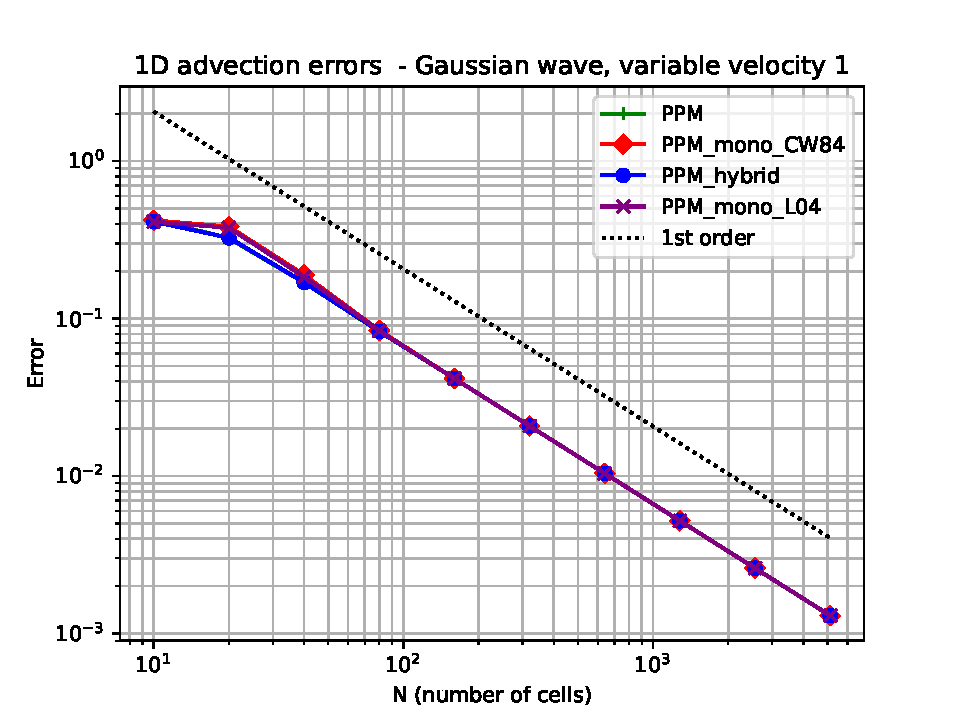
\includegraphics[width=1\linewidth]{1d_adv_tc2_ic2_vf2_parabola_errors}
		\caption{Error.\label{chp2-sec-exp-adv4-error}}
  \end{subfigure}
  \begin{subfigure}{0.49\textwidth}
    \centering
			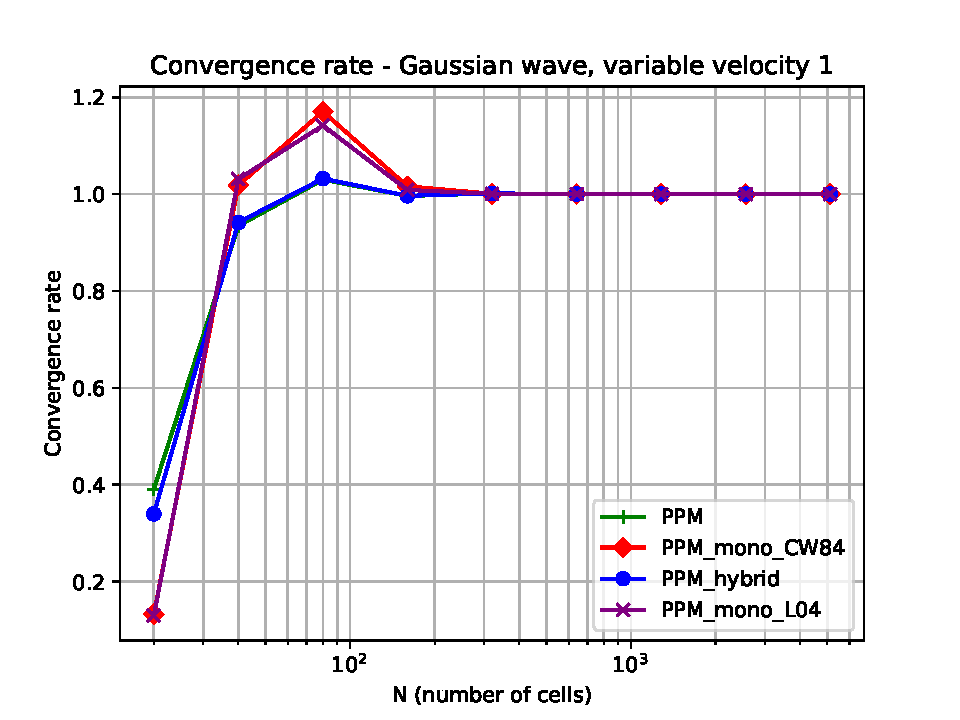
\includegraphics[width=1\linewidth]{1d_adv_tc2_ic2_vf2_convergence_rate}
		\caption{Convergence rate.\label{chp2-sec-exp-adv4-CR}}
  \end{subfigure}
	\caption{ Similar to Figure \ref{chp2-sec-exp-adv1-2} but using
	the initial condition given by Equation	\eqref{chp2-ic2} and the variable 
	velocity given by Equation \eqref{chp2-vel1}.\label{chp2-sec-exp-adv4-2}}
\end{figure}



\newpage

\begin{figure}[!htb]
  \centering
  \begin{subfigure}{0.49\textwidth}
    \centering
			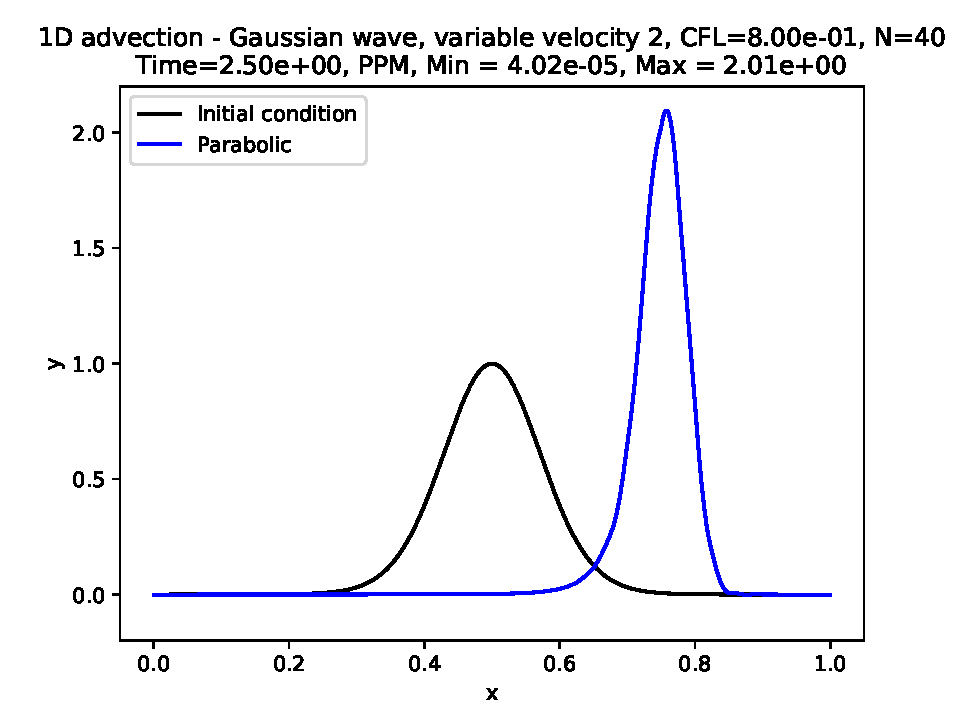
\includegraphics[width=1\linewidth]{1d_adv_tc2_ic2_vf3_t24_N40_PPM}
			\caption{PPM.\label{chp2-sec-exp-adv5-a}}
  \end{subfigure}
  \begin{subfigure}{0.49\textwidth}
    \centering
			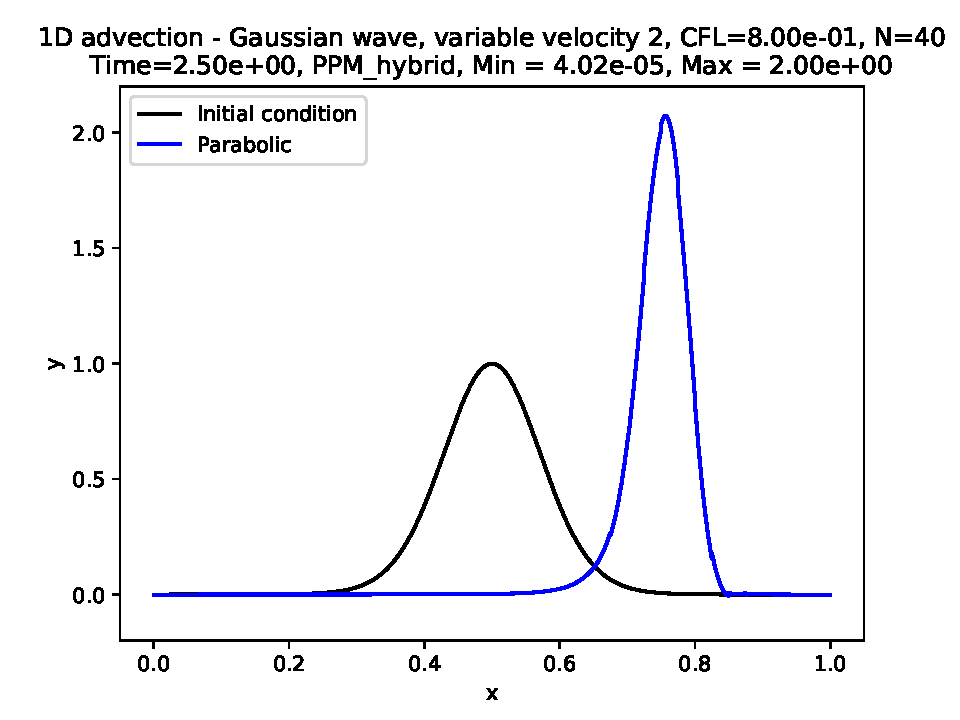
\includegraphics[width=1\linewidth]{1d_adv_tc2_ic2_vf3_t24_N40_PPM_hybrid}
			\caption{Hybrid PPM.\label{chp2-sec-exp-adv5-b}}
  \end{subfigure}

  \begin{subfigure}{0.49\textwidth}
    \centering
		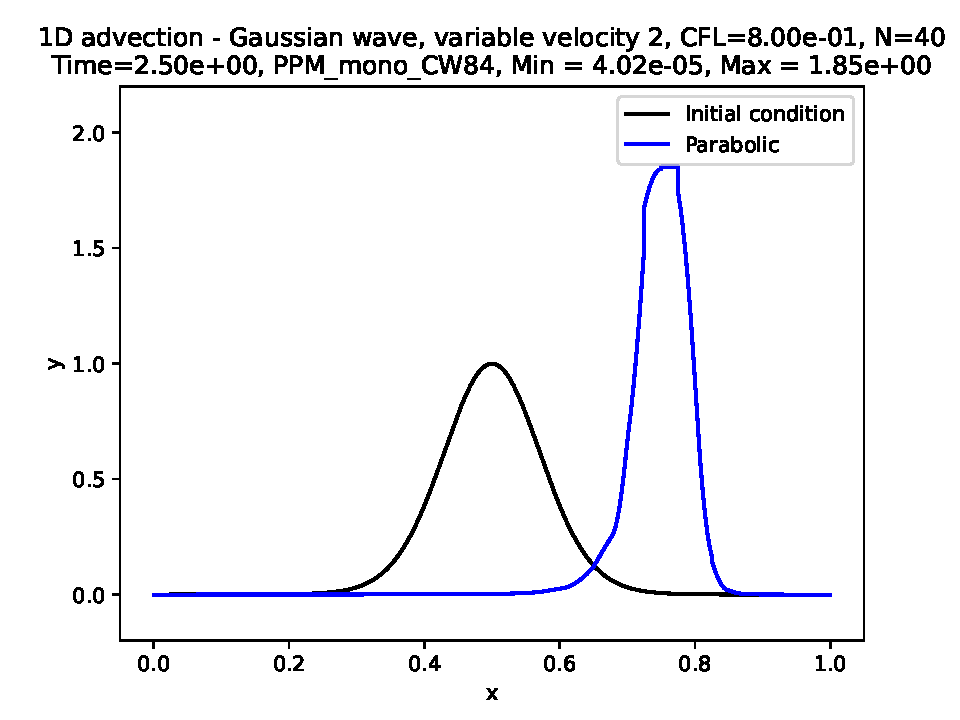
\includegraphics[width=1\linewidth]{1d_adv_tc2_ic2_vf3_t24_N40_PPM_mono_CW84}
    \caption{PPM + CW84 monotonization.\label{chp2-sec-exp-adv5-c}}
  \end{subfigure}
  \begin{subfigure}{0.49\textwidth}
    \centering
			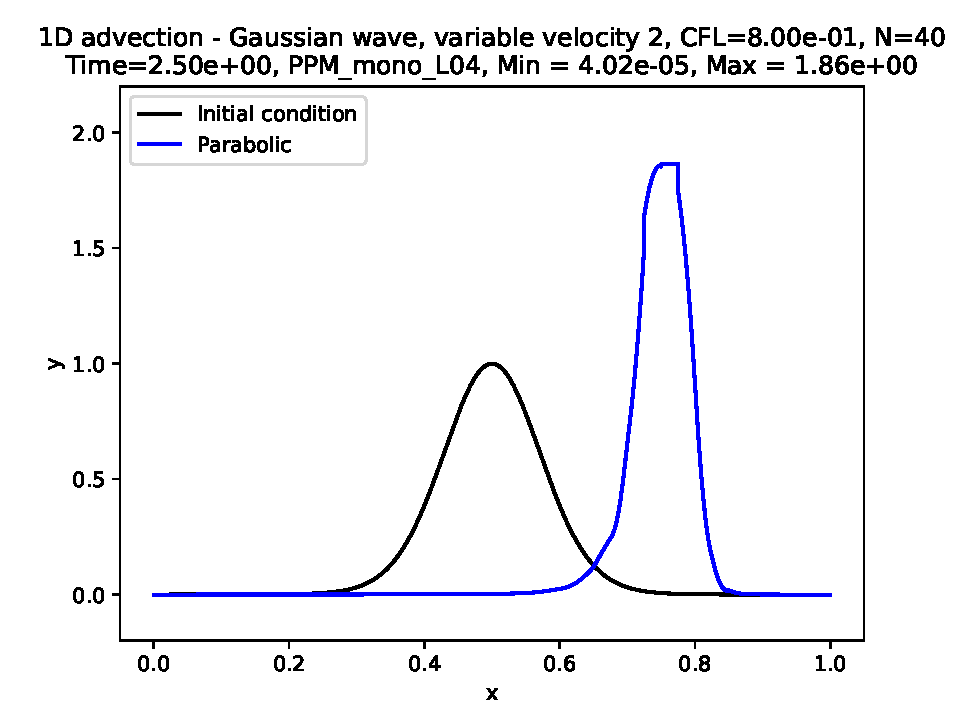
\includegraphics[width=1\linewidth]{1d_adv_tc2_ic2_vf3_t24_N40_PPM_mono_L04}
      \caption{PPM + L04 monotonization.\label{chp2-sec-exp-adv5-d}}
  \end{subfigure} 

  \begin{subfigure}{0.49\textwidth}
    \centering
			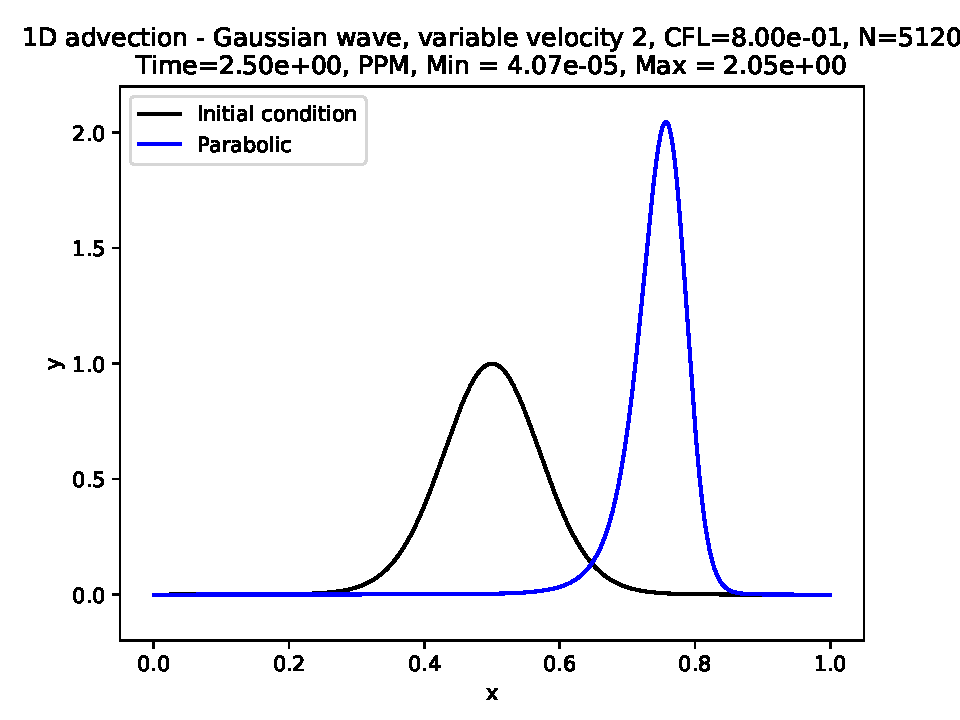
\includegraphics[width=1\linewidth]{1d_adv_tc2_ic2_vf3_t3199_N5120_PPM}
      \caption{Reference solution.\label{chp2-sec-exp-adv5-e}}
  \end{subfigure} 
	\caption{ Similar to Figure \ref{chp2-sec-exp-adv1} but using $N=40$, 
	the initial condition given by Equation \eqref{chp2-ic2}, the variable velocity given by Equation
	\eqref{chp2-vel2} and the final time is 2.5 (half a period). In (e) we show a reference solution, using the PPM scheme with 
	5120 cells. \label{chp2-sec-exp-adv5}}
\end{figure}

\newpage


\begin{figure}[!htb]
  \centering
  \begin{subfigure}{0.49\textwidth}
    \centering
			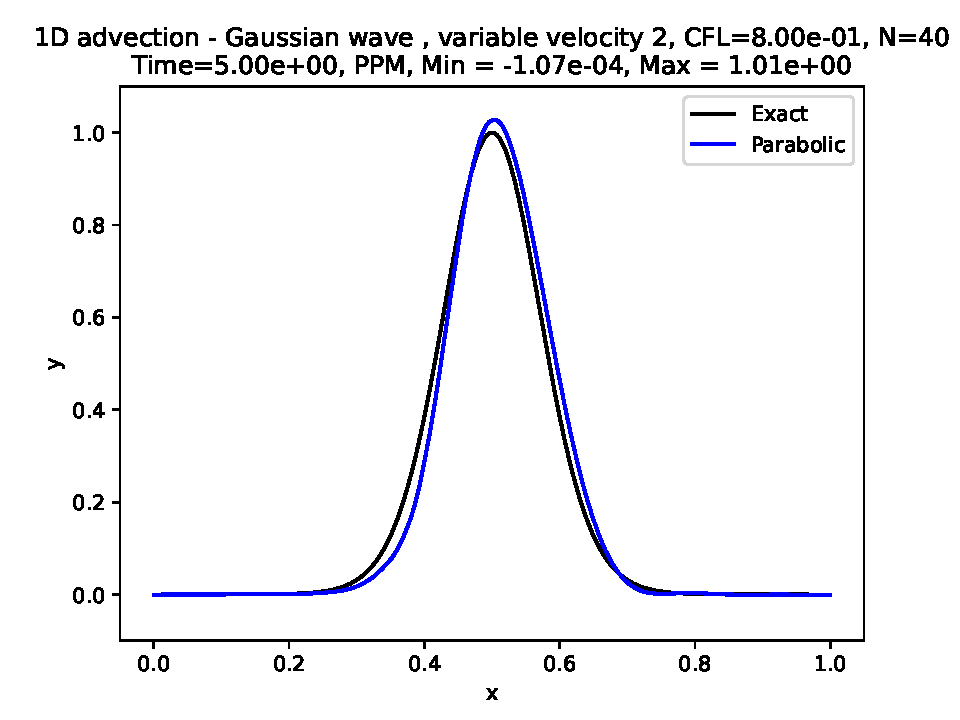
\includegraphics[width=1\linewidth]{1d_adv_tc2_ic2_vf3_t49_N40_PPM}
			\caption{PPM.\label{chp2-sec-exp-adv6-a}}
  \end{subfigure}
  \begin{subfigure}{0.49\textwidth}
    \centering
			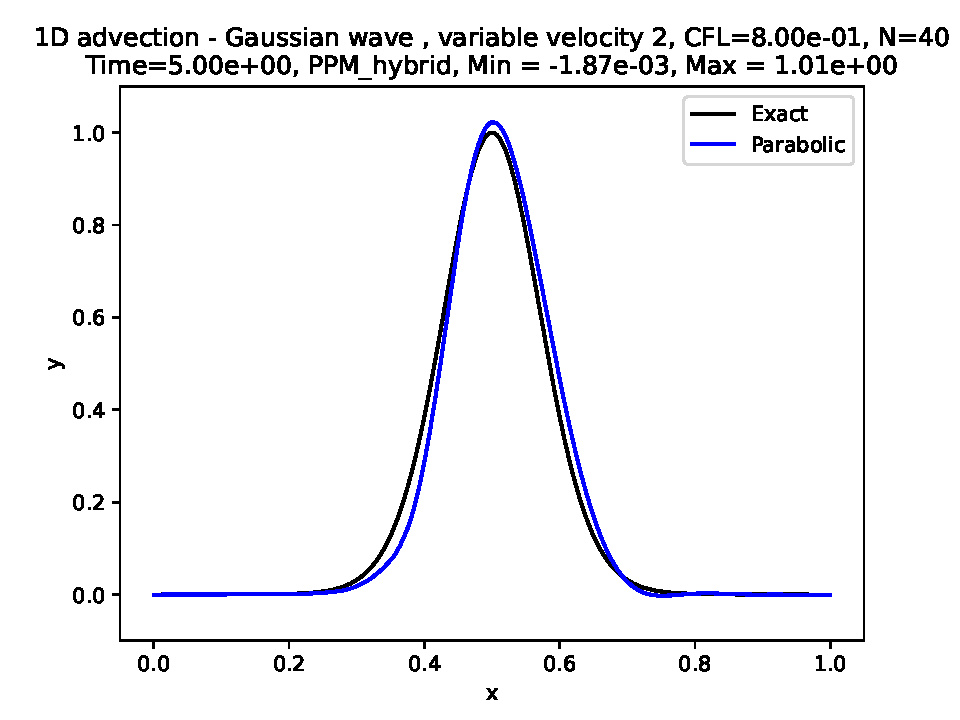
\includegraphics[width=1\linewidth]{1d_adv_tc2_ic2_vf3_t49_N40_PPM_hybrid}
			\caption{Hybrid PPM.\label{chp2-sec-exp-adv6-b}}
  \end{subfigure}

  \begin{subfigure}{0.49\textwidth}
    \centering
		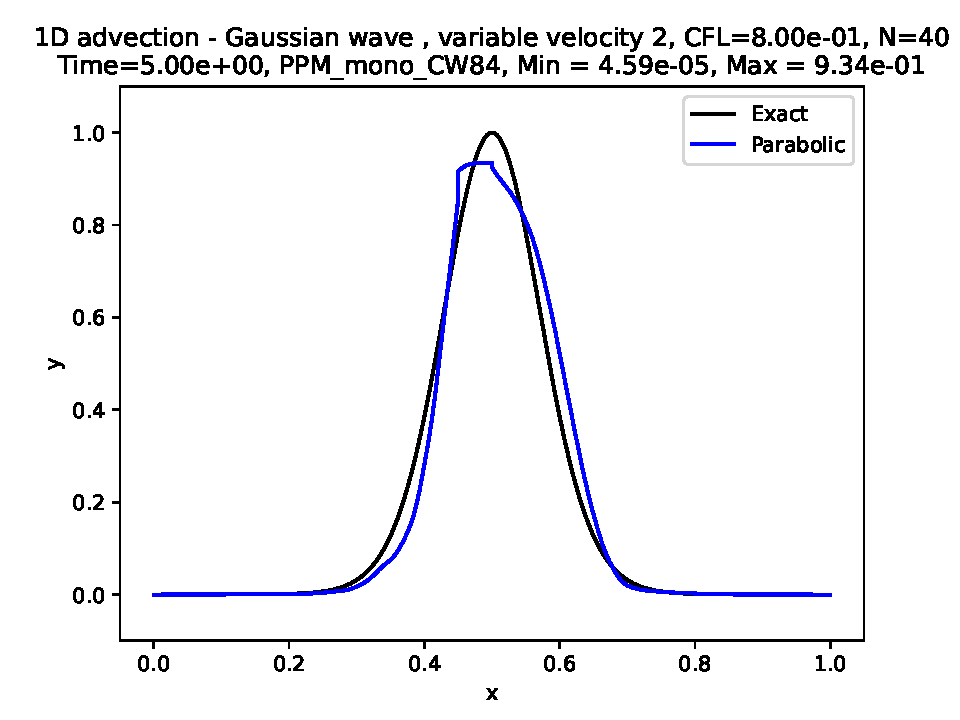
\includegraphics[width=1\linewidth]{1d_adv_tc2_ic2_vf3_t49_N40_PPM_mono_CW84}
    \caption{PPM + CW84 monotonization.\label{chp2-sec-exp-adv6-c}}
  \end{subfigure}
  \begin{subfigure}{0.49\textwidth}
    \centering
			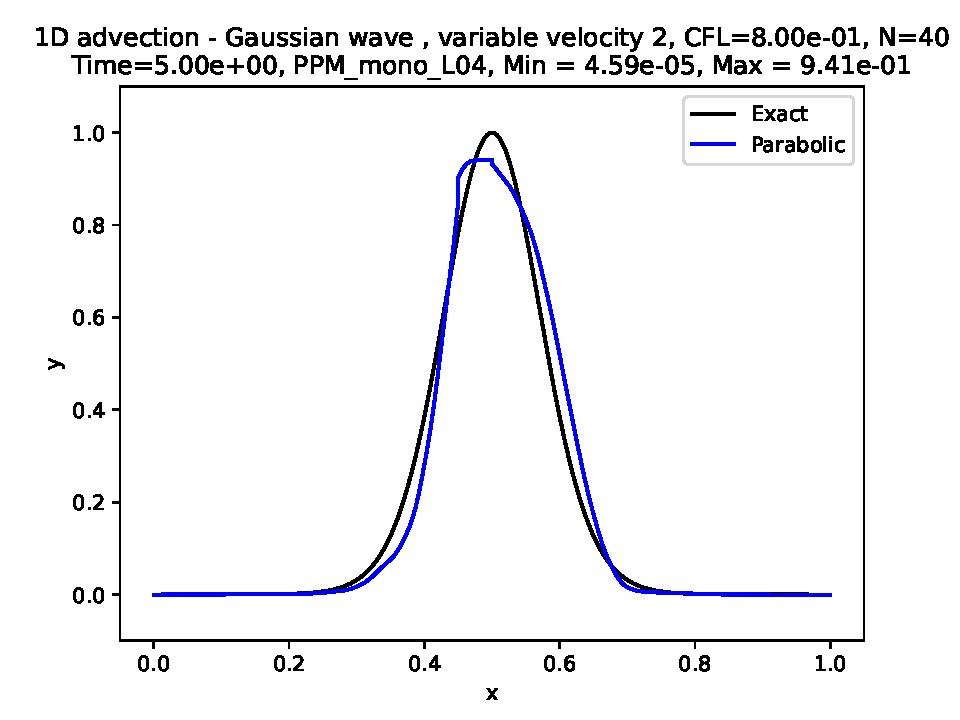
\includegraphics[width=1\linewidth]{1d_adv_tc2_ic2_vf3_t49_N40_PPM_mono_L04}
      \caption{PPM + L04 monotonization.\label{chp2-sec-exp-adv6-d}}
  \end{subfigure} 
	\caption{ Similar to Figure \ref{chp2-sec-exp-adv2} but using $N=40$, 
	the initial condition given by Equation \eqref{chp2-ic2} and the variable velocity given by Equation
	\eqref{chp2-vel2} \label{chp2-sec-exp-adv6}.}
\end{figure}

\begin{figure}[!htb]
  \centering
  \begin{subfigure}{0.49\textwidth}
    \centering
		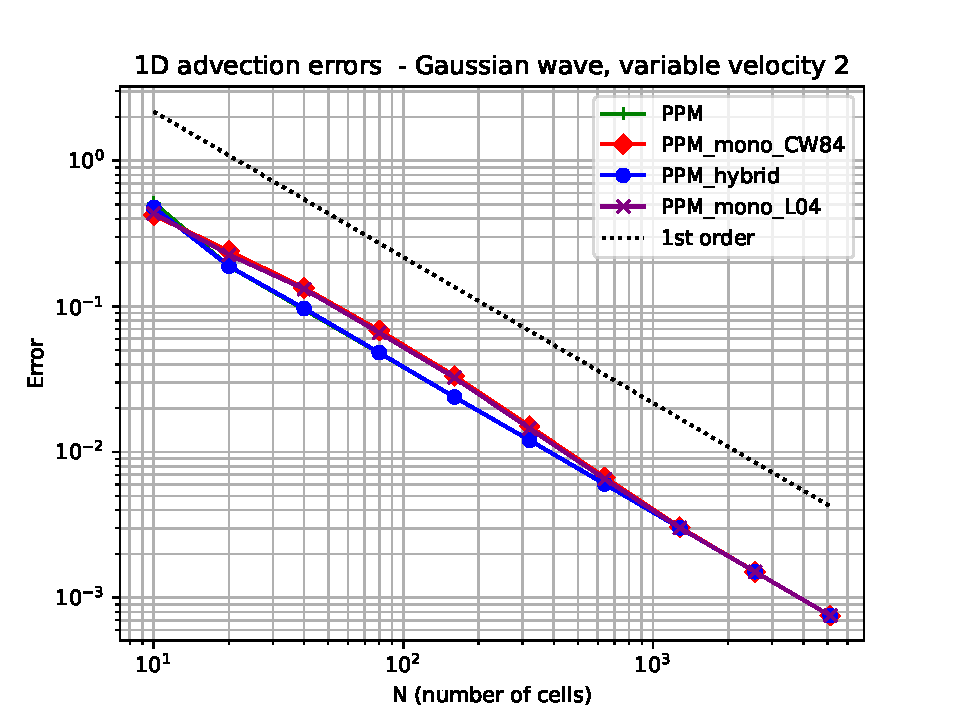
\includegraphics[width=1\linewidth]{1d_adv_tc2_ic2_vf3_parabola_errors}
		\caption{Error.\label{chp2-sec-exp-adv6-error}}
  \end{subfigure}
  \begin{subfigure}{0.49\textwidth}
    \centering
			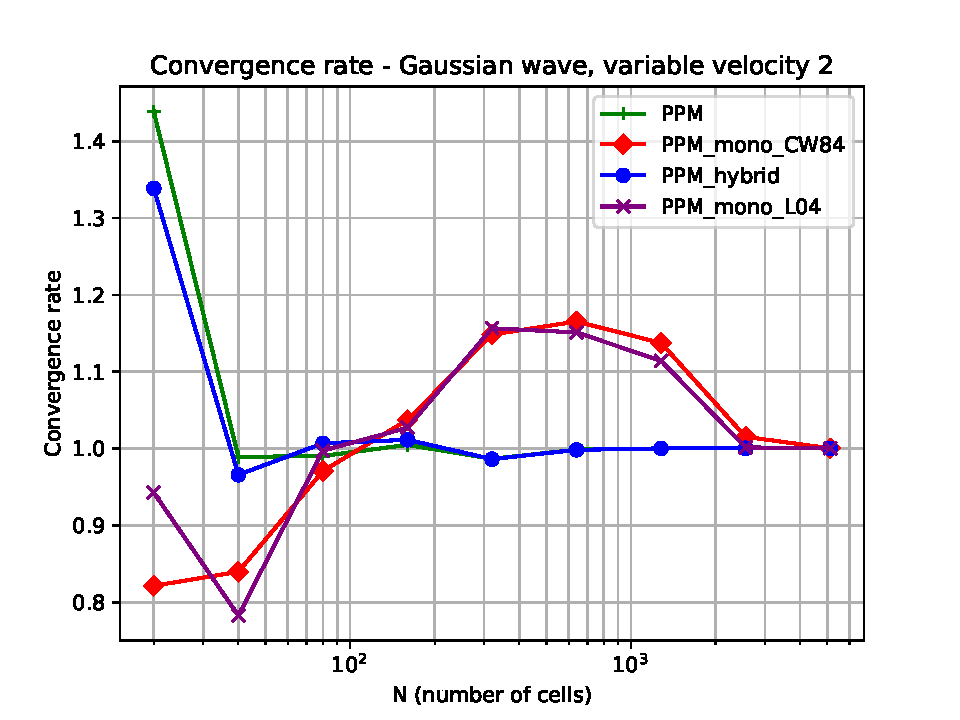
\includegraphics[width=1\linewidth]{1d_adv_tc2_ic2_vf3_convergence_rate}
		\caption{Convergence rate.\label{chp2-sec-exp-adv6-CR}}
  \end{subfigure}
	\caption{ Similar to Figure \ref{chp2-sec-exp-adv1-2} but using
	the initial condition given by Equation	\eqref{chp2-ic2} and the variable 
	velocity given by Equation \eqref{chp2-vel2}.\label{chp2-sec-exp-adv6-2}}
\end{figure}

\newpage
\section{Concluding remarks}
\label{chp2-sec-conclusion}